\documentclass[oneside]{scrartcl}
\usepackage[english]{babel}
\usepackage[utf8]{inputenc}
\usepackage[usenames,dvipsnames]{color}
\usepackage{amsmath}
\usepackage{amssymb}
\usepackage{amstext}
\usepackage{amsthm}
\usepackage{thmtools}
\usepackage{enumerate}
\usepackage{enumitem}
\usepackage{listings}
\usepackage{caption}
\usepackage[automark]{scrpage2}
\usepackage[section]{algorithm}
\usepackage{algorithmicx}
\usepackage{algpseudocode}
\usepackage{tikz}
\usepackage{pgfplots}
\usetikzlibrary{calc,trees,positioning,arrows,chains,shapes.geometric,%
    decorations.pathreplacing,decorations.pathmorphing,shapes,%
    matrix,shapes.symbols,positioning}
\usetikzlibrary{fit}
\usetikzlibrary{backgrounds}
\usepackage[bottom=10em]{geometry}
\usepackage{booktabs}
\usepackage{multirow}
\usepackage{array}

%%%%%%%%%%%%%%%%%%%%%%%%%%%%%%%%%%%%%%%%%%%%%%%%%%%%%%%%%%%%%%%%%%%%%%%%%%%%%%%
% STYLES
%%%%%%%%%%%%%%%%%%%%%%%%%%%%%%%%%%%%%%%%%%%%%%%%%%%%%%%%%%%%%%%%%%%%%%%%%%%%%%%

\tikzset{
  %nodes
  Inst/.style={
    rectangle,
    draw=black!80,
    fill=black!40,
    rounded corners,
    inner sep=0.2em,
    minimum height=2em,
    minimum width=8em,
    thick,
    font=\sffamily
  },
  %edges
  thick edge/.style={-latex,very thick,shorten >=2pt,shorten <=2pt,line cap=round},
  thin edge/.style={-latex,thin,shorten >=1pt,shorten <=1pt,line cap=round},
  scheddep/.style={thick edge,blue},
  datadep/.style={thin edge,black},
  begin2end/.style={thick edge,dashed},
  cfg/.style={thick edge},
  %background
  basicblock/.style={fill=black!10,inner sep=0.5em,thick,rectangle,rounded corners},
}

% instructions
\newcommand{\Inst}[1]{#1}

\renewcommand{\heavyrulewidth}{1pt}

\newcolumntype{L}[1]{>{\raggedright\let\newline\\\arraybackslash\hspace{0pt}}m{#1}}
\newcolumntype{C}[1]{>{\centering\let\newline\\\arraybackslash\hspace{0pt}}m{#1}}
\newcolumntype{R}[1]{>{\raggedleft\let\newline\\\arraybackslash\hspace{0pt}}m{#1}}

\numberwithin{figure}{section}
\numberwithin{table}{section}

\newcommand{\irinline}[1]{\textsf{#1}}

\lstset{
language=Java,
keywordstyle=\bfseries,
basicstyle=\sffamily\small,
columns=flexible,
captionpos=b,
caption=~,
mathescape=true,
tabsize=4,
belowcaptionskip=8pt
}

% caption style for listings
\captionsetup[lstlisting]{
singlelinecheck=false,
margin=0pt,
labelfont={bf,normalsize,sf},
labelsep=space,
font={small},
justification=justified
}

% caption style for algorithms
\captionsetup[algorithm]{
singlelinecheck=false,
margin=0pt,
labelfont={bf,normalsize,sf},
labelsep=space
}

% caption style for figures
\captionsetup[figure]{
singlelinecheck=true,
margin=0pt,
format=plain,
labelfont={bf,normalsize,sf},
%font={small},
labelsep=space,
justification=justified,
minmargin=0.05\textwidth
}

% caption style for tables
\captionsetup[table]{
singlelinecheck=true,
margin=0pt,
format=plain,
labelfont={bf,normalsize,sf},
labelsep=space,
justification=justified,
minmargin=0.05\textwidth
}

% the title and style of the abstract part
\renewcommand{\abstractname}{}
\renewenvironment{abstract}{
  \begin{center}
  \textbf{\Large\rmfamily Abstract}\\[10pt]
 
  \begin{minipage}{0.9\textwidth}
  \itshape
}{\end{minipage}
\end{center}}

% style for the header line of the content pages
\renewcommand{\headfont}{\rmfamily\MakeUppercase}

% theorem style for definitions
\declaretheoremstyle[
  headfont=\sffamily\bfseries,
]{definitionstyle}

% theorem type for definitions
\declaretheorem[
  name=Definition,
  numberwithin=section,
  style=definitionstyle
]{definition}

% theorem style for lemmas
\declaretheoremstyle[
  headfont=\sffamily\bfseries,
]{claimstyle}

% theorem type for definitions
\declaretheorem[
  name=Claim,
  numberwithin=section,
  style=claimstyle
]{claim}

% bibliography style
\bibliographystyle{alpha}

\AtBeginDocument{%
\renewcommand{\thealgorithm}{\thesection .\arabic{algorithm}}
\numberwithin{lstlisting}{section}
}

% Define bar chart colors
\definecolor{bblue}{HTML}{4F81BD}
\definecolor{rred}{HTML}{C0504D}
\definecolor{ggreen}{HTML}{9BBB59}
\definecolor{ppurple}{HTML}{9F4C7C}

\newcommand{\barwidth}{6pt}
\newcommand{\barpadding}{0.4pt}
\newcommand{\chartheight}{9cm}
\newcommand{\enlargexlimits}{0.06}

%%%%%%%%%%%%%%%%%%%%%%%%%%%%%%%%%%%%%%%%%%%%%%%%%%%%%%%%%%%%%%%%%%%%%%%%%%%%%%%
% BODY
%%%%%%%%%%%%%%%%%%%%%%%%%%%%%%%%%%%%%%%%%%%%%%%%%%%%%%%%%%%%%%%%%%%%%%%%%%%%%%%

\begin{document}

% empty 
\pagestyle{scrheadings}
\clearscrheadfoot

\begin{titlepage}

\newcommand{\HRule}{\rule{\linewidth}{0.5mm}} % Defines a new command for the horizontal lines, change thickness here

\center % Center everything on the page
 
\vspace*{60pt} 
 
%----------------------------------------------------------------------------------------
%	HEADING SECTIONS
%----------------------------------------------------------------------------------------

\textsc{\LARGE Bachelor's Thesis}\\[1.5cm]

%----------------------------------------------------------------------------------------
%	TITLE SECTION
%----------------------------------------------------------------------------------------

\HRule \\[0.3cm]
{\LARGE \bfseries SSA-based Optimizations for\\[2pt]Just-in-Time Compilation in the CACAO VM}\\[0.3cm] % Title of your document
\HRule \\[1.5cm]

\textsc{\Large Vienna University of Technology}\\[0.5cm]
\textsc{\large Institute of Computer Languages\\Compilers and Languages Group}\\[2cm]

%----------------------------------------------------------------------------------------
%	DATE SECTION
%----------------------------------------------------------------------------------------

{\large \today}

%----------------------------------------------------------------------------------------
%	AUTHOR SECTION
%----------------------------------------------------------------------------------------

\vfill

\begin{flushleft} \large
\emph{Author:}\\
Matthias \textsc{Reisinger} % Your name
\end{flushleft}

\begin{flushleft} \large
\emph{Supervisor:} \\
Ao.Univ.Prof.\ Dipl.-Ing.\ Dr.techn Andreas \textsc{Krall} % Supervisor's Name
\end{flushleft}

\end{titlepage}
\begin{abstract}
The CACAO VM is a virtual machine for the native execution of Java bytecode based on just-in-time compilation. Since bytecode interpretation is not applied, a fast compiler performs the initial compilation tasks to translate a Java program to machine code. Due to the need of short compilation time, exhaustive optimizations are not employed at this level. Subsequently, those parts of the program which are executed frequently have to be recompiled using a higher level of optimization. At the time this work is written, a new version of the compiler framework for performing these recompilation tasks is implemented for future integration into the CACAO VM. Prior to optimization, this framework translates the program into a high-level intermediate representation based on static single assignment form. The subject of this work is to examine machine independent optimization techniques and how to apply them to this intermediate representation respectively. The according considerations serve as the basis for implementation and incorporation into the new compiler. Concretely, the techniques called dead code elimination, constant folding, constant propagation and global value numbering have been subject to examination and have been realized accordingly. An empirical analysis of these optimizations discloses the effects of incorporating them into the new compiler.
\end{abstract}

\tableofcontents
\newpage

\pagestyle{scrheadings}
\clearscrheadfoot
\ihead[]{\textsc{\headmark}}
\ohead[\pagemark]{\pagemark}
\setheadsepline[\textwidth]{0.5pt}

\section{Introduction}
\label{sec:introduction}

\subsection{The CACAO VM}
\label{sec:the-cacao-vm}

The CACAO VM is a virtual machine for executing Java bytecode. Instead of interpreting this bytecode, just-in-time compilation is used to execute Java programs natively. Consequently, the first time a part of a program, or a method respectively, has to be executed by the virtual machine, the so called \emph{baseline} compiler will directly translate it to native machine code, which is invoked subsequently. Short compilation time is required at this level, therefore exhaustive optimization tasks cannot be taken into account. As a consequence, for those program parts which are executed very often, the machine code produced at this level will not provide adequate efficiency in general. The run-time behavior of the program will be profiled in the following, to identify those methods which are executed more frequently. The according program parts will then be recompiled by comprising in-depth optimization tasks to produce efficient native code eligible for frequent execution. This approach is referred to as \emph{adaptive optimization}. At present, these recompilation tasks are also achieved by the baseline compiler, but differently, at this level the compiler applies additional optimization techniques to meet the according efficiency requirements.

\subsection{Motivation}
\label{sec:motivation}

Due to reasons of maintenance and the need of a higher flexibility concerning the integration of new optimization techniques, the baseline compiler will be replaced as optimizing compiler. Therefore a new compiler will be incorporated into the CACAO VM, which performs the according tasks in the course of adaptive optimization. Currently this compiler is subject to implementation and is not yet fully operational, also in-depth optimizations have to be integrated.

\subsection{Aim of the Work}
\label{sec:aim}

The subject of this thesis is to examine machine independent optimizations and how to apply them to the SSA-based intermediate representation used within the new compiler framework. These examinations form the basis for their implementation and integration into the compiler.
Due to the fact that the compilation tasks are performed during run-time of the virtual machine, efficient algorithms are required so that fast execution of the optimizations is possible.

\subsection{Structure of the Thesis}
\label{sec:paper-structure}

Section \ref{sec:intermediate-representation} gives a basic introduction to the intermediate representation used in the new compiler framework. In sections \ref{sec:dead-code}, \ref{sec:constantprop} and \ref{sec:global-value-numbering} we describe the optimization techniques we examined for the use within the compiler. For each of the optimizations there will be given a description of its goals and general characteristics. The last part of each of these sections is formed by exhaustive explanations of how the optimizations can be applied to the intermediate representation, enclosed by algorithms formally describing how these techniques can be realized. The effects of incorporating them into the compiler are discussed in section \ref{sec:evaluation}, where the results of the empirical evaluation are presented.
In section \ref{sec:related} we give an overview of alternative approaches and describe how they are different from the presented techniques.
The last part of the thesis is formed by section \ref{sec:conclusions} which outlines the central findings of our work.

\section{The Intermediate Representation}
\label{sec:intermediate-representation}

The new optimizing compiler of the CACAO VM uses two different forms of intermediate representations for the code \cite{eisl:2013}. A high-level representation model, based on static single assignment form, builds the center of the architecture independent parts. Later on, within the architecture dependent compiler back-end, this structure is transformed into a low-level representation, which uses lists of machine instructions to form basic blocks. The optimization algorithms presented in subsequent sections are targeted at being incorporated into the machine independent front-end of the compiler and operate on the high-level representation. In the following, we will give an overview of its main characteristics because basic knowledge about it is necessary for a thorough understanding of the optimization algorithms. We will not go into detail on every aspect, so for further information refer to \cite{eisl:2013}.

As already mentioned, this intermediate representation is based on static single assignment form. It represents a method's code in the form of a graph-based structure, where instructions are represented by nodes. Each node has an associated type, which is part of a static type hierarchy. Each type is a direct or indirect sub-type of \irinline{Instruction}, which forms the base of this hierarchy. In the following, we will use the terms \emph{node} and \irinline{Instruction} interchangeably (similarly, to refer to nodes associated with a sub-type of \irinline{Instruction}, we will use the according type name). The possible relationships between nodes are represented by three different types of edges: \emph{control-flow edges}, \emph{data-flow edges} and \emph{scheduling edges}.

The units of control-flow within this graph are the nodes of type \irinline{BEGINInst} and \irinline{ENDInst}. These nodes form pairs which are comparable to basic blocks in traditional representation models. But as we will see later on, in contrast to basic blocks, there do not necessarily exist lists of instructions which are assigned to these control-flow units. On one hand, at \irinline{BEGINInsts} several control-flow paths merge, meaning that there can be a number of control-flow edges, that go into a node of this type. Each \irinline{BEGINInst} will have a single outgoing edge leading to exactly one \irinline{ENDInst}. On the other hand, these \irinline{ENDInst}s can have several outgoing control-flow edges to \irinline{BEGINInst}s. There are different sub-types of \irinline{ENDInst}: \irinline{GOTOInst}s, for example, which can only have a single outgoing edge, or \irinline{IFInst}s with two outgoing edges; another important example are nodes of type \irinline{RETURNInst}, which do not have outgoing edges at all.

\begin{lstlisting}[label=lst:factorial, caption=Example adopted from \cite{eisl:2013}]
static long fact(long n) {
	long res = 1;
	while(1 < n) {
		res *= n--;
	}
	return res;
}
\end{lstlisting}

Besides these units to express the program's control-flow, there are also primitive nodes that compute and supply data values. They can have multiple inputs, namely their operands, which are represented by ordered incoming data-flow edges. The value computed by such nodes can be consumed and serve as operand for other nodes. The latter case is modeled by using data-flow edges starting at the supplying node and ending at the consuming one. A special case of such nodes are those which represent $\phi$-functions. These \irinline{PHIInst}s serve to merge values at points where multiple control-flow paths join. Each $\phi$-node is fixed to exactly one \irinline{BEGINInst} and accordingly has to be scheduled after this node. Such dependencies are modeled by using scheduling edges which define the order of execution between nodes. Although there exist some explicit scheduling dependencies like in the case of $\phi$-nodes, an important aspect of this intermediate representation is that there does not exist a complete instruction schedule.

The method in listing \ref{lst:factorial} would be translated into this intermediate representation as can be seen in figure \ref{fig:ir-demo}.

\begin{figure}[H]
\centering
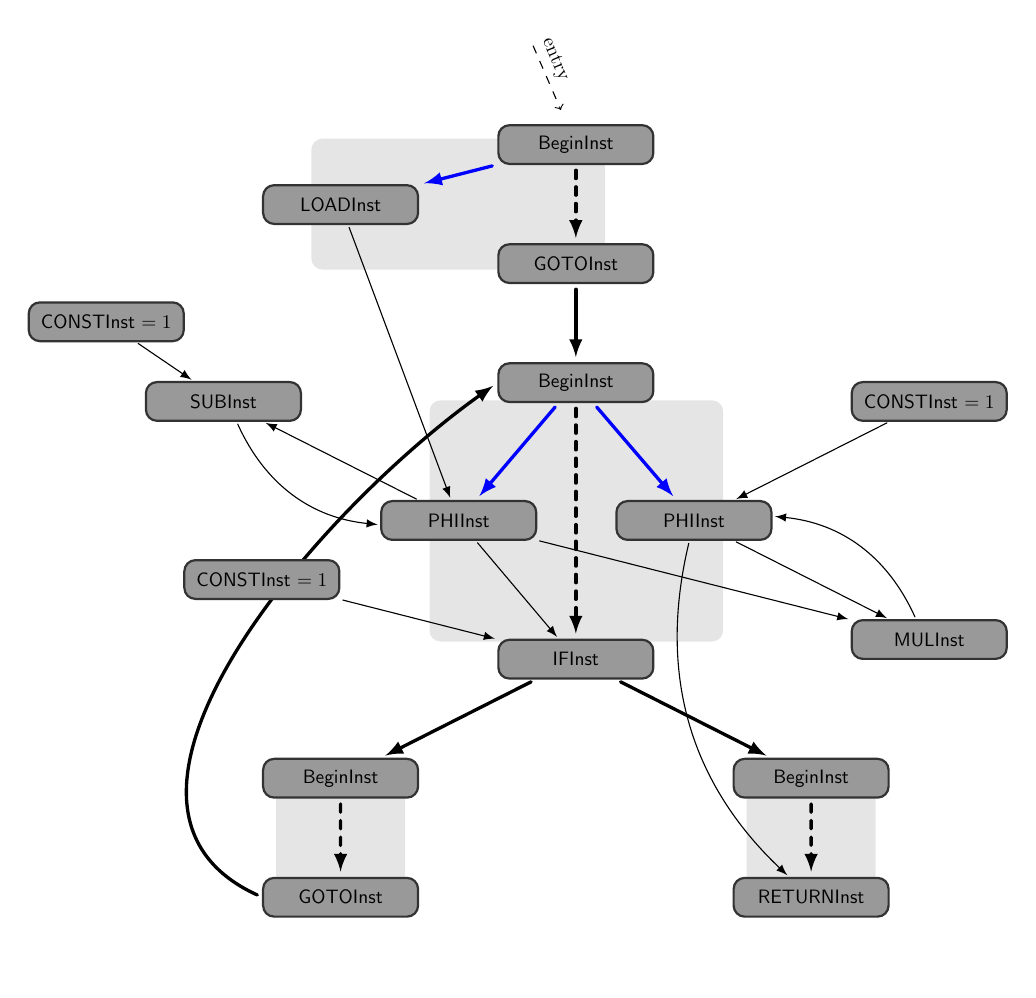
\begin{tikzpicture}%
[
  scale=0.7,
  every node/.style={
   scale=0.7
 },
  %show background rectangle,
  %inner frame sep=1em,
]
%[scale=0.4]
%
  %\draw[step=.5cm,black!25,very thin,draw opacity=1] (-3,-3) grid (3,3);
 
  %%
  \node[Inst] (begin0) {\Inst{BeginInst}};
 \node[Inst] (goto6) [below=of begin0] {\Inst{GOTOInst}};
 \node (start) [above left=1 and -0.5 of begin0] {};
  %
  \node[Inst] (load4) [below left= 0.25 and 1 of begin0] {\Inst{LOADInst}};
  %%
  \node[Inst] (begin1) [below=of goto6] {\Inst{BeginInst}};
 \node[Inst] (if9) [below=3 of begin1] {\Inst{IFInst}};
  %
  \node[Inst] (phi8) [above left=1.25 and -0.5  of if9] {\Inst{PHIInst}};
 \node[Inst] (phi10) [right=of phi8] {\Inst{PHIInst}};
 \node[Inst] (mul13) [below right=of phi10] {\Inst{MULInst}};
 \node[Inst] (const5) [above right=of phi10] {\Inst{CONSTInst} $=1$};
 \node[Inst] (const7) [above left=0.5 and 2 of if9] {\Inst{CONSTInst} $=1$};
  %%
  \node[Inst] (begin2) [below left=of if9] {\Inst{BeginInst}};
 \node[Inst] (goto14) [below=of begin2] {\Inst{GOTOInst}};
  %%
  \node[Inst] (begin3) [below right=of if9] {\Inst{BeginInst}};
 \node[Inst] (return15) [below=of begin3] {\Inst{RETURNInst}};
  %%
  \node[Inst] (sub12) [above left=of phi8] {\Inst{SUBInst}};
 \node[Inst] (const11) [above left= 0.5 and - 0.5 of sub12] {\Inst{CONSTInst} $=1$};
  %
  \node[below=0.5 of return15] {};
  %%
  \begin{pgfonlayer}{background}
   \node[basicblock,fit=(begin0) (goto6) (load4)] {};
   \node[basicblock,fit=(begin1) (if9) (phi8) (phi10)] {};
   \node[basicblock,fit=(begin2) (goto14)] {};
   \node[basicblock,fit=(begin3) (return15)] {};
 \end{pgfonlayer}
  %%
  % begin end
  \draw [dashed,->,shorten >=0.2cm] (start) to node[sloped,anchor=south,near start] {entry} (begin0);
  \draw [begin2end] (begin0) to (goto6);
  \draw [begin2end] (begin1) to (if9);
  \draw [begin2end] (begin2) to (goto14);
  \draw [begin2end] (begin3) to (return15);
  % data dep
  \draw [datadep] (const5) to (phi10);
  \draw [datadep] (const7) to (if9);
  \draw [datadep] (phi8) to (if9);
  \draw [datadep] (load4) to (phi8);
  \draw [datadep,bend right] (phi10) to (return15);
  \draw [datadep] (const11) to (sub12);
  \draw [datadep] (phi8) to (sub12);
  \draw [datadep,bend right] (sub12) to (phi8);
  \draw [datadep] (phi8) to (mul13);
  \draw [datadep] (phi10) to (mul13);
  \draw [datadep,bend right] (mul13) to (phi10);
  % sched dep
  \draw [scheddep] (begin0) to (load4);
  \draw [scheddep] (begin1) to (phi8);
  \draw [scheddep] (begin1) to (phi10);
  % cfg
  \draw [cfg] (goto6) to (begin1);
  \draw [cfg] (if9) to (begin2);
  \draw [cfg] (if9) to (begin3);
  \begin{pgfonlayer}{background}
   \draw [cfg,bend left] (goto14.west) to [out=90] (begin1.west);
 \end{pgfonlayer}
\end{tikzpicture}
\caption{Control-flow is marked by thick solid arrows. To highlight pairs of \irinline{BEGINInst}s and \irinline{ENDInst}s, the according edges are dashed. Data-flow is represented by thin arrows pointing into def-use direction. Scheduling dependencies are marked blue. Example adopted from \cite{eisl:2013}}
\label{fig:ir-demo}
\end{figure}
\section{Dead Code Elimination}
\label{sec:dead-code}

The term \emph{dead code elimination} has originally been used to refer to two separate optimization techniques, namely \emph{unused code elimination} and \emph{unreachable code elimination} \cite{wegman:1991:constantpropagation}. Despite its title, this section is targeted only at the first of these two techniques. The examinations and algorithms for unused code elimination, which we are describing here, are mainly based on considerations in \cite{appel:2004:moderncompilerimpl}, where the notion of dead code elimination is used as a synonym for this technique. Thus we will also prefer the according term to refer to this optimization.

The goal of this technique can be described intuitively by the idea to remove all those code sections from the program, whose results are never used. Assuming that the program, which is subject to dead code elimination, satisfies the property of static single assignment form, a characterization of \emph{dead} variables can be given:
\begin{definition}\label{def:dead-variable}
A variable is \emph{dead} if and only if its list of uses is empty and its assignment statement has no side effects.
\end{definition}

It is further assumed that each statement in the program or in the according intermediate representation is an ordinary assignment, an assignment using a $\phi$-function, a fetch, store or branch \cite{appel:2004:moderncompilerimpl}. Based on these considerations and on definition \ref{def:dead-variable} the idea of this optimization can be characterized by the following short algorithm:

\begin{algorithm}
\caption{Basic idea of dead code elimination}
\label{alg:dead-basic}
\begin{algorithmic}[1]
\While{there is a \emph{dead} variable $v$}
  \State{remove $v$'s defining statement from the program}
\EndWhile
\end{algorithmic}
\end{algorithm}

At each iteration, the algorithm removes one statement which defines a dead variable. Furthermore, the affected statement has to be removed from the use lists of those variables which are referenced within such a defining assignment. This in turn can cause these variables to become dead, which will be handled in subsequent iterations.

\subsection{Application to the Intermediate Representation}
\label{sec:dead-code:application-to-the-ir}

As mentioned earlier, the intermediate representation of the new compiler satisfies the property of static single assignment form. Nevertheless, it does not contain statements or variables in the traditional sense, instead it uses nodes to express data-flow and control-flow within the program. Therefore, it is not possible to directly apply the definition of dead variables to optimize this graph-based structure. But based on previous considerations, definition \ref{def:dead-node} gives a characterization of dead nodes (it explicitly excludes control-flow nodes, as they do not represent data computations and thus do not supply values for consumption by other nodes).

\begin{definition}\label{def:dead-node}
A node, which does not mark control-flow, is \emph{dead} if and only if its list of uses is empty, it has no side effects and there are no other dependencies on that node.
\end{definition}

\begin{algorithm}
\caption{Basic idea of dead code elimination on the intermediate representation}
\label{alg:dead-ir-basic}
\begin{algorithmic}[1]
\While{there is a \emph{dead} node $n$}
  \State{remove node $n$ from the graph}
\EndWhile
\end{algorithmic}
\end{algorithm}

Based on the notion of dead nodes, it is now possible to translate the idea of dead code elimination accordingly as shown in algorithm \ref{alg:dead-ir-basic}. This pseudo code leaves many details open and is not meant as a reference for implementation. Therefore, algorithm \ref{alg:dead-ir} gives a more formal formulation for dead code elimination which is based on \cite{appel:2004:moderncompilerimpl}. It iteratively removes dead nodes from the graph. On that account it uses a work list $\mathcal{W}$, which before every iteration of the while-loop contains all those nodes that have to be reconsidered by the algorithm. Despite this container is called ``work list'', it is not important whether the underlying data structure is organized as a list or as another container type. The only aspects to consider are, that the removal in line \ref{alg:dead-ir:W-remove} is done in constant time and that the insertion at line \ref{alg:dead-ir:W-add} (represented by the union operation) avoids to add duplicates, assuming a constant time membership check on the container (in fact it would also be possible to handle duplicates when removing nodes from the work list). At every iteration of the while-loop a node that has to be reconsidered is removed from the work list, to examine if it is dead and thus should be deleted from the program. Every time a node is identified to be dead, it will also be deleted from the list of uses of all the operand nodes, referenced by the dead node. Thus, in turn each of these nodes has to be reconsidered because its own list of uses can have become empty now and hence is added to the work list.

\begin{algorithm}[H]
\caption{Dead code elimination}
\label{alg:dead-ir}
\begin{algorithmic}[1]
\State $\mathcal{W} \gets$ all nodes in the intermediate representation graph\label{alg:dead-ir:W-init}
\While{$\mathcal{W}$ is not empty}
	\State remove some node $n$ from $\mathcal{W}$\label{alg:dead-ir:W-remove}
	\If{$n$ is \emph{dead}}
		\For{each node $x_i$ used by $n$}
			\State delete $n$ from the list of uses of $x_i$\label{alg:dead-ir:op-remove}
			\State $\mathcal{W} \gets \mathcal{W} \cup \lbrace x_i\rbrace$\label{alg:dead-ir:W-add}
		\EndFor
	\EndIf
\EndWhile
\end{algorithmic}
\end{algorithm}

The general running time of this algorithm is linear in the size of the intermediate representation graph. Each time a node is removed from the work list and discovered dead, each of its operands will be visited (the number of operands of any node is equivalent to the number of use-def edges starting at that node). In case the node is not dead, the amount of work which is done is constant. An aspect that could lead to an increase of the asymptotic run-time complexity of this algorithm is the deletion of nodes from the use lists of their operands in line \ref{alg:dead-ir:op-remove}. Therefore, a data structure that allows constant time removal should be used for the realization of the use lists.
\section{Constant Folding \& Propagation}
\label{sec:constantprop}

In general, constant folding and constant propagation are techniques that optimize programs by performing transformations on those code parts that make use of values which are statically known to be constant. The reason to cover these optimizations within only one section and not devote a single one to each of them is, that they can be combined very effectively.

Constant folding, also known as constant expression evaluation, evaluates those expressions at compile-time, for which each operand is a constant value \cite{muchnick:1997:advanced-compiler-design}. That means, computations that would have been done during run-time are now executed during the compilation process. It is important, that the result of this compile-time computation has to be the same as the one that would have been computed during the execution of the compiled program. Thus it is necessary to consider all those aspects that could cause a difference between the result of a static evaluation and that of the run-time evaluation of an expression. For example, if the floating point representation or the floating point arithmetic of the compiler deviates from the run-time environment of the compiled program, this could lead to differing results of the according computations. Another aspect to consider is that exceptional cases --- like divisions by zero --- have to be handled accordingly.

% TODO: introducing phrase for constant propagation
Assuming a program or intermediate representation is in static single assignment form, the general idea of constant propagation can be described by the following rule \cite{appel:2004:moderncompilerimpl}: For any assignment of the form $v \leftarrow c$ for some constant $c$, replace each use of the variable $v$ by $c$. Nevertheless, this rule ignores an important case, namely the occurrence of $\phi$-functions, for which an additional rule has to be considered \cite{appel:2004:moderncompilerimpl}: Any $\phi$-function of the form $v \leftarrow \phi (x_1, x_2,\ldots , x_n)$, where all $x_i$ are equal to some constant $c$, can be replaced by $v \leftarrow c$. An iterative application of these rules can now be used to propagate constants as far as possible through a program. The principles of constant propagation considered so far, describe a restricted form of this type of optimization. In section \ref{sec:related} we will thus shortly present an extension of this optimization technique which combines constant propagation with unreachable code elimination and therefore discovers additional optimization possibilities.

What is left to say is that constant folding, on the one hand, can lead to code that can be further optimized by the use of constant propagation. The application of constant propagation, on the other hand, can lead to code that in turn can be further optimized by the use of constant folding. For example, the expression on the right-hand side of the assignment statement in listing \ref{lst:const-combined} can be evaluated leading to the code in listing \ref{lst:const-combined-opt1}. This provides the further possibility to propagate the constant value of variable \lstinline!a! to the return statement in the next line. This in turn yields further folding possibilities as can be seen in listing \ref{lst:const-combined-opt2}, where the operation within the return statement only uses constant operands.

\newsavebox{\lstConstCombined}
\begin{lrbox}{\lstConstCombined}
\begin{lstlisting}[label=lst:const-combined]
a = 1 + 2;
return a + 3;
\end{lstlisting}
\end{lrbox}

\newsavebox{\lstConstCombinedFirstOpt}
\begin{lrbox}{\lstConstCombinedFirstOpt}
\begin{lstlisting}[label=lst:const-combined-opt1]
a = 3;
return a + 3;
\end{lstlisting}
\end{lrbox}

\newsavebox{\lstConstCombinedSecondOpt}
\begin{lrbox}{\lstConstCombinedSecondOpt}
\begin{lstlisting}[label=lst:const-combined-opt2]
a = 3;
return 3 + 3;
\end{lstlisting}
\end{lrbox}

\begin{minipage}[b]{0.33\textwidth}
\centerline{\usebox{\lstConstCombined}}
\end{minipage}
~
\begin{minipage}[t]{0.34\textwidth}
\centerline{\usebox{\lstConstCombinedFirstOpt}}
\end{minipage}
~
\begin{minipage}[t]{0.33\textwidth}
\centerline{\usebox{\lstConstCombinedSecondOpt}}
\end{minipage}

Obviously, the rules for constant propagation, defined earlier, lead to dead code, as shown in listing \ref{lst:const-combined-opt2}, where variable \lstinline!a! is not referenced anymore. A run of dead code elimination, as described in section \ref{sec:dead-code}, can be used to eliminate the unused code.

\subsection{Application to the Intermediate Representation}
\label{sec:constantprop:application-to-the-ir}

Due to the characteristics of the intermediate representation of the compiler framework, constant propagation will be an implicit effect of constant folding. Each node with constant operands that represents an operation that can be evaluated statically (like arithmetical or logical operations) will be replaced by introducing a new node of type \irinline{CONSTInst}. The value of this constant node will be the result of the original node's operation, applied to the values of its operands. Furthermore, each node that references the replaced node as an operand has to adjust the according references within its use list to point to the newly introduced node. The replacement of nodes in the course of the folding deletes all the references to them, thus they become dead according to definition \ref{def:dead-node} in section \ref{sec:dead-code:application-to-the-ir}. A subsequent run of dead code elimination at the end of this optimization would delete these dead nodes.

To illustrate the application of constant folding, we will reconsider the example code from listing \ref{lst:const-combined}, but we first have to translate it into the intermediate representation (for reasons of simplicity, the following figures will not include the dead nodes that would reside within the program). Figure \ref{fig:const-combined} shows the graph, which is the result of this translation.

\vspace{3pt}
\begin{figure}[H]
\centering
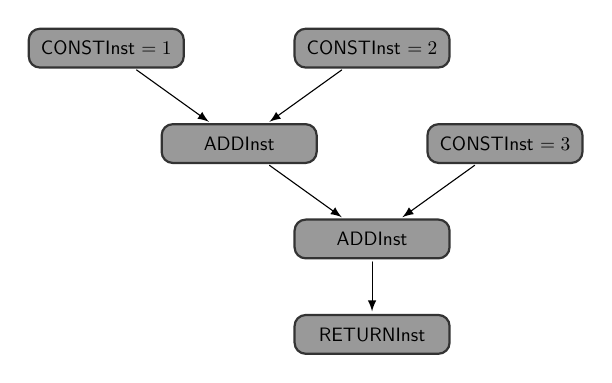
\begin{tikzpicture}[every node/.style={scale=0.7, node distance=0.7cm and -0.3cm}]
  \node[Inst] (return) [] {\Inst{RETURNInst}};
  \node[Inst] (add1) [above=of return] {\Inst{ADDInst}};
  \node[Inst] (const1) [above right=of add1] {\Inst{CONSTInst} $=3$};
  \node[Inst] (add2) [above left=of add1] {\Inst{ADDInst}};
  \node[Inst] (const2) [above left=of add2] {\Inst{CONSTInst} $=1$};
  \node[Inst] (const3) [above right=of add2] {\Inst{CONSTInst} $=2$};

  % data dep
  \draw [datadep] (add1) to (return);
  \draw [datadep] (const1) to (add1);
  \draw [datadep] (add2) to (add1);
  \draw [datadep] (const2) to (add2);
  \draw [datadep] (const3) to (add2);
\end{tikzpicture}
\caption{}
\label{fig:const-combined}
\end{figure}

The topmost node of type \irinline{ADDInst} in this graphic represents the expression \lstinline!1 + 2!, having only constant operands. Thus, it can be evaluated and replaced by a new node of type \irinline{CONSTInst} whose value corresponds to the result of this operation. Figure \ref{fig:const-combined-opt1} presents the graph after the according transformation. The remaining \irinline{ADDInst} now has only operands of type \irinline{CONSTInst}. Thus, it can be folded further and replaced by a new constant node, leading to the graph in figure \ref{fig:const-combined-opt2}.

\vspace{3pt}
\begin{figure}[H]
\begin{minipage}[b]{0.5\textwidth}
\centering
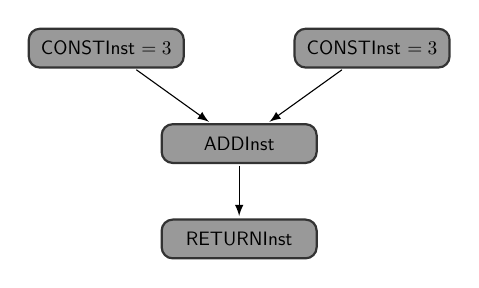
\begin{tikzpicture}[every node/.style={scale=0.7, node distance=0.7cm and -0.3cm}]
  \node[Inst] (return) [] {\Inst{RETURNInst}};
  \node[Inst] (add1) [above=of return] {\Inst{ADDInst}};
  \node[Inst] (const1) [above right=of add1] {\Inst{CONSTInst} $=3$};
  \node[Inst] (const2) [above left=of add1] {\Inst{CONSTInst} $=3$};
  % data dep
  \draw [datadep] (add1) to (return);
  \draw [datadep] (const1) to (add1);
  \draw [datadep] (const2) to (add1);
\end{tikzpicture}
\caption{}
\label{fig:const-combined-opt1}
\end{minipage}
~
\begin{minipage}[b]{0.5\textwidth}
\centering
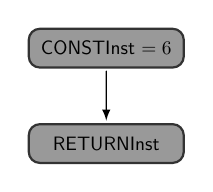
\begin{tikzpicture}[every node/.style={scale=0.7, node distance=0.7cm and -0.3cm}]
  \node[Inst] (return) [] {\Inst{RETURNInst}};
  \node[Inst] (const) [above=of return] {\Inst{CONSTInst} $=6$};
  % data dep
  \draw [datadep] (const) to (return);
\end{tikzpicture}
\caption{}
\label{fig:const-combined-opt2}
\end{minipage}
\end{figure}

These examples illustrate how the propagation of constants is done implicitly when introducing the new constant nodes during folding. The only places where propagation has to be done explicitly, are occurrences of nodes which represent $\phi$-functions. The following rule covers this case: Each node of type \irinline{PHIInst}, for which all operands are equal to some constant $c$, can be replaced by introducing a new node of type \irinline{CONSTInst}, whose value is set to $c$.

\begin{algorithm}[t]
\caption{Combined constant folding \& propagation}
\label{alg:const-ir}
\begin{algorithmic}[1]
\State $\mathcal{W} \gets$ all nodes in the intermediate representation graph
\While{$\mathcal{W}$ is not empty}
	\State remove some node $n$ from $\mathcal{W}$
	\If{all operands $o_i$ of node $n$ are constant}\label{alg:const-ir:operand-check}
		\If{$n$ is of type PHIInst and all $o_i$ are equal to some constant value $c$}\label{alg:const-ir:operand-check-equal}
			\State \Call{ReplaceByConstant}{n, c}
		\ElsIf{$n$'s operation can be evaluated statically}\label{alg:const-ir:if-evaluatable}
			\State $x \gets$ the result of $n$'s operation applied to $n$'s operands\label{alg:const-ir:cont-init}
			\State \Call{ReplaceByConstant}{n, x}
		\EndIf
	\EndIf
\EndWhile
\end{algorithmic}
\end{algorithm}

Based on the previous considerations, a more detailed formulation of this combined version of constant folding and constant propagation is given in algorithm \ref{alg:const-ir}. It is an adaption of a constant propagation algorithm described by Appel and Palsberg \cite{appel:2004:moderncompilerimpl} and revisits the idea of using a work list for those nodes that should be reconsidered, like it already has been done for dead code elimination in section \ref{sec:dead-code:application-to-the-ir}. We again assume constant time removal and the avoidance of duplicate entries in this container. At each iteration of the while loop a node will be removed from the work list to consider if all of its operands are constant nodes. According to the previously defined rules, we then have to further distinguish if the node is of type \irinline{PHIInst} or if it represents any other operation that can be evaluated at compile-time. The steps that have to be done during the according node replacements have been outsourced to a procedure whose pseudo code is shown in algorithm \ref{alg:const-ir-replace}.

In general, the execution of the condition test in line~\ref{alg:const-ir:operand-check} of algorithm~\ref{alg:const-ir} would involve to examine the node's whole operand list. Nevertheless, it is possible to implement this test to be executed in constant time. One possibility would be to keep a counter for each node, whose value represents the number of operands which are constants. Each time a \irinline{CONSTInst} is added to the node's operand list, the counter will be increased. Accordingly, each time a \irinline{CONSTInst} is removed from the operand list, the counter will be decreased. Thus if all the operands of a node are constant, then this counter would be equal to the number of operands. The condition test could then be realized by a comparison of the counter to the size of the operand list.

The running time of the presented algorithm is in $\mathcal{O}(E\cdot O + N)$ where $E$ is the number of data-flow edges in the graph, $O$ is the maximum number of operands of any node and $N$ is the number of nodes in the program. We will constitute this in the following.

Each time a node is replaced by a new constant node (and obviously each node can be replaced at most once), we will have to examine all of its users which is done by following each def-use edge that starts at that node. Consequently, the maximum number of data-flow edges which will be visited in def-use direction during the whole algorithm is obviously limited by $E$. For each of the users, it is necessary to inspect the whole operand list, to replace all the references to the original node by a reference to the new constant node. This takes time linear to the size of the corresponding operand list, which is limited by $O$. Each user will then be placed on the work list for reconsideration.
In the following, if one of these nodes is removed from the work list, the condition test in line \ref{alg:const-ir:operand-check} of algorithm \ref{alg:const-ir} will be performed, which, with respect to previous considerations, can be done in constant time (this test is actually performed at least $N$ times, since at the beginning of the algorithm, the work list contains all the nodes in the program).
The algorithm will again pass through a node's operand list in line \ref{alg:const-ir:operand-check-equal}, when determining if all operands represent the same constant value, which again is limited by $O$.

\begin{algorithm}[t]
\caption{Procedure for node replacements}
\label{alg:const-ir-replace}
\begin{algorithmic}[1]
\Procedure{ReplaceByConstant}{$n_{\mathit{old}}$, $c$}
	\State create a new constant node $n_{\mathit{new}}$\label{alg:cont-ir:create-const}
	\State $n_{\mathit{new}}.\mathit{value} \gets c$\label{alg:const-ir:cont-init}
	\For{each user $u_i$ of $n_{\mathit{old}}$}\label{alg:const-ir:for-loop-users}
		\State replace each occurrence of $n_{old}$ in $u_i$'s list of operands by $n_{\mathit{new}}$\label{alg:const-ir:replace-operand}
		\State $\mathcal{W} \gets \mathcal{W} \cup \lbrace u_i\rbrace$\label{alg:const-ir:worklist-insert}
	\EndFor
\EndProcedure
\end{algorithmic}
\end{algorithm}

\section{Global Value Numbering}
\label{sec:global-value-numbering}

The equivalence of programs or the equivalence of expressions that are part of programs is undecidable in general \cite{alpern:1988:detecting-equality-of-variables}. Despite this impossibility to formulate an algorithm that finds all the equivalences in a program, there exist optimization techniques that identify certain sub classes of these equivalencies. One of these techniques is \emph{global value numbering}, which finds and removes redundant computations.

This optimization discovers redundancies by assigning \emph{value numbers} to expressions based on their specific operation and the value numbers of their operands. Subsequently, all those occurrences of expressions that have been assigned the same value number, can then be replaced by a single one, thus eliminating redundant computations. As the name already suggests, this whole process is not restricted to the bounds of basic blocks, namely, it is applied in a global manner. There are several ways to realize this optimization which can generally be categorized into two approaches. The pessimistic approach, on the one hand, initially assumes that all expressions are different by assigning distinct value numbers to them. It then continues by trying to find expressions that can be proven to be equivalent and allots equal value numbers to them. On the other hand, the optimistic approach initially assumes that all expressions --- or specific subsets thereof --- are the same and will then refine this assumption. The algorithm which we formulated for integration into the compiler follows the optimistic approach, therefore we will not go into further detail on the pessimistic one.
\newpage
Basically, global value numbering detects equal variables or expressions based on their \emph{congruence}, which is a weaker property than equality. More specifically, if two expressions are congruent, this also implies that they are equal but the reverse does not hold in general (an explanation of this relation between these properties will be given when we describe how to apply these concepts to nodes within our intermediate representation). Basically, two operations are said to be \emph{congruent} if they use equal function symbols on congruent operands. With a few exceptions, which will be explained later on, this denotes the main characterization of this notion. 

Optimistic global value numbering initially proceeds by creating sets of expressions which are supposed to be possibly congruent. For example, all arithmetical operations that use the same function symbol will be combined in a set. These sets can be referred to as \emph{blocks} which are all part of the current \emph{partition}. As long as it can be shown that some block contains expressions which are not congruent, the according blocks will be split up and the partition will be refined until each of its blocks contains only congruent expressions. When this refinement terminates, the result will be a final partition of blocks of expressions that are known to compute equal values at run-time. Based on this classification, it is then possible to remove redundant computations. The whole process of this approach is outlined in figure \ref{fig:gvn-schema}, dividing this optimization into three steps, which have just been described.

\begin{center}
\begin{minipage}{0.65\textwidth}
\begin{figure}[H]
\centering
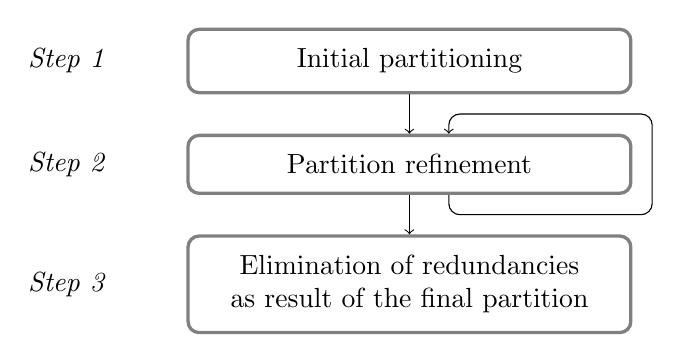
\begin{tikzpicture}
[step-node/.style={
	rectangle,
	rounded corners,
	draw=black!50,
	very thick,
	inner sep=7pt,
	minimum width=160pt,
	node distance=0.5cm and 0.5cm,
	align=center},
step-label/.style={
	rectangle,
	rounded corners,
	draw=white,
	inner sep=0pt,
	outer sep=0pt,
	minimum width=1pt,
	align=center}]
	
  \node[step-node] (initial) {Initial partitioning};
  \node[step-label] (initial-label) [left=of initial] {\textit{Step 1}};
  \node[step-node] (partitioning) [below=of initial] {Partition refinement};
  \node[step-label] (partitioning-label) [left=of partitioning] {\textit{Step 2}};
  \node[step-node] (consolidate) [below=of partitioning] {Elimination of redundancies\\ as result of the final partition};
  \node[step-label] (consolidate-label) [left=of consolidate] {\textit{Step 3}};
  % edges
  \draw [->] (initial) to (partitioning);
  \draw [->] (partitioning) to (consolidate);
  \draw [->,rounded corners]
  					($ (partitioning.south) + (5mm,0) $)
  					-- ++(0,-2.5mm)
  					-| ($ (partitioning.east) + (2.5mm,0) $)
  					|- ($ (partitioning.north) + (5mm,2.5mm) $)
  					-- ($ (partitioning.north) + (5mm,0) $);
\end{tikzpicture}
\caption{A schematic overview of the optimistic global value numbering approach. Figure adopted from \cite{kongstad:2004:gnu-gvn}.}
\label{fig:gvn-schema}
\end{figure}
\end{minipage}
\end{center}

\subsection{Application to the Intermediate Representation}
\label{sec:global-value-numbering:application-to-the-ir}

The algorithm that we have formulated for the application within the compiler follows the optimistic global value numbering approach and is based on the principles described above. Instead of expressions, the blocks will now contain nodes. Accordingly, at the end of the partition refinement, all nodes in a block can be replaced by a single congruent one. But before going into detail on the algorithm, the notion of congruence has to be defined in terms of our intermediate representation. We have already given a very abstract characterization of this property which based the congruence of two operations on the equality of their function symbols and the congruence of their operands. But so far, this ignores that some operations need special care, like $\phi$-functions or operations without any operands, etc. For example, in the case of $\phi$-functions whose according operands have been proven to be all congruent, it is not possible to consolidate them in general. An additional aspect has to be taken into account, namely, to be congruent they also have to reside in the same basic block. Based on the considerations of Click \cite{click:1995:combininganalyses} and Alpern et al. \cite{alpern:1988:detecting-equality-of-variables} we define congruence as done in the following.

\begin{definition}
\label{def:congruent}
Two nodes are \emph{congruent} if and only if they are identical or one of the following statements holds:
\begin{itemize}
\item Both nodes are \irinline{CONSTInst}s and represent the same constant value.
\item Both nodes are \irinline{PHIInst}s which are assigned to the same \irinline{BEGINInst} and for each $i$ it holds that the operands at index $i$ of the nodes' operand lists are \emph{congruent}.
\item Both nodes are of the same type and for each $i$ it holds that the operands at index $i$ of the nodes' operand lists are \emph{congruent} but neither node is of type \irinline{CONSTInst}, \irinline{PHIInst}, \irinline{BEGINInst} or \irinline{ENDInst} nor does it have an effect on or depends on the global state.
\end{itemize}
\end{definition}

As formulated in definition \ref{def:congruent}, congruence not only depends on the type of the operation but also on the order of the operands. This means that two operations like \lstinline!x + y! and \lstinline!y + x! would not be considered congruent, even though they would produce equal outputs. Therefore, this example illustrates that equality not necessarily implies congruence as already mentioned before.

According to previous descriptions, the creation of the initial partition, in terms of our intermediate representation, consists in combining possibly congruent nodes into blocks. The generation of these sets is based on several assumptions which are reflected in the following basic rules:

\begin{itemize}
\item All \irinline{CONSTInst}s  which represent the same constant value are combined into a common block.
\item All \irinline{PHIInst}s which are assigned to the same \irinline{BEGINInst} are combined into a common block.
\item Each node which has an effect on or depends on the global state will go into a separate block.
\item All other nodes which are neither \irinline{BEGINInst}s nor \irinline{ENDInst}s will be merged into blocks depending on their node type, i.e., all nodes of the same type will share a block.
\end{itemize}

The subsequent refinement of this partition is comparable to the partitioning when minimizing a finite automaton, where states are initially partitioned into final and non-final states. Based on the state transitions in the automaton, the initial partition will be improved until it contains only sets of equal states. Hopcroft \cite{hopcroft:1971:an-n-log-n-algorithm} gave an algorithm which solves this problem in $\mathcal{O}(k\cdot n\cdot \mathit{log}(n))$ where $n$ is the number of states and $k$ is the number of symbols in the input alphabet of the according automaton.
Reformulations of the original algorithm that have been presented by Berstel et al. \cite{berstel:2010:minimization-of-automata} and Click \cite{click:1995:combininganalyses} form the basis of our approach listed in algorithm \ref{alg:gvn-ir}.
It corresponds to the second step in figure \ref{fig:gvn-schema} (the third and last step in this schema has already been explained earlier in this section and the according considerations stay the same when applied to the nodes of the intermediate representation).

\begin{algorithm}[h]
\caption{Global Value Numbering -- Partition Refinement}
\label{alg:gvn-ir}
\begin{algorithmic}[1]
\State $\mathcal{P} \leftarrow$ initial partition
\State $\mathcal{W} \leftarrow \emptyset$
\For{each $P \in \mathcal{P}$}\label{alg:gvn-ir:init-worklist-loop}
  \For{$i = 1,\ldots ,O$}
    \State $\mathcal{W} \leftarrow \mathcal{W}~\cup (P, i)$
  \EndFor
\EndFor
\While{$\mathcal{W}$ is not empty}
  \State remove some tuple $(W,i)$ from $\mathcal{W}$
  \State $\mathit{split\_ candidates} \leftarrow \emptyset$
  \For{each node $x \in W$}
    \For{each node $y \in x.\mathit{def\_ use}_i$}\label{alg:gvn-ir:touched-nodes-loop}
      \State $\mathit{split\_ candidates} \leftarrow \mathit{split\_ candidates}~ \cup ~ \lbrace y.\mathit{block}\rbrace$ % TODO: duplicates
      \State $y.\mathit{block}.\mathit{touched} \leftarrow y.\mathit{block}.\mathit{touched}~ \cup ~ \lbrace y\rbrace$
    \EndFor
  \EndFor
  \For{each partition $X$ in $\mathit{split\_ candidates}$}
    \If{$|X| \neq |X.\mathit{touched}|$}\label{alg:gvn-ir:if-test-split-touched}
      \State \Call{Split}{$X$}
    \EndIf
    \State $X.\mathit{touched} \leftarrow \emptyset$
  \EndFor
\EndWhile
\end{algorithmic}
\end{algorithm}

\begin{algorithm}[h]
\caption{Pseudo code for block splitting}
\label{alg:gvn-ir-split}
\begin{algorithmic}[1]
\Procedure{Split}{$P$}
  \State remove all nodes in $P.\mathit{touched}$ from $P$\label{alg:gvn-ir:remove-touched-nodes-from-block}
  \State move $P.\mathit{touched}$ to a new block $P'$\label{alg:gvn-ir:move-touched-nodes-to-new-block}
  \State $\mathcal{P} \leftarrow \mathcal{P}~\cup ~\lbrace P'\rbrace$\label{alg:gvn-ir:add-new-block-to-partition}
  \For{$j = 1,\ldots ,O$}\label{alg:gvn-ir:split-loop}
    \If{$(P,j) \not\in \mathcal{W}$ and $|P| \leq |P'|$}
      \State $\mathcal{W} \leftarrow \mathcal{W} \cup \lbrace (P,j)\rbrace$
    \Else
      \State $\mathcal{W} \leftarrow \mathcal{W} \cup \lbrace (P',j)\rbrace$
    \EndIf
  \EndFor
\EndProcedure
\end{algorithmic}
\end{algorithm}

The algorithm uses a work list, which contains pairs of the form $(W,i)$ where $W$ stands for a block of nodes and $i$ designates an operand index. The initialization of this list is done in the loop starting at line \ref{alg:gvn-ir:init-worklist-loop} (in the next line and the rest of the algorithm, $O$ stands for the maximum size of any node's operand list). For each block which is part of the initial partition and each operand index in the given range, there will be placed such a pair on the work list. Each time one of these tuples $(W,i)$ is removed from the list, the algorithm will mark each block, which contains at least one node, whose operand at index $i$ is part of $W$. On that account, all these blocks are gathered in the set $\mathit{split\_ candidates}$ (the notion $x.\mathit{def\_ use}_i$ on line \ref{alg:gvn-ir:touched-nodes-loop} designates the set of nodes which use $x$ as their $i$th operand). Accordingly, for each of these ``split candidates'' we have to remember all of its nodes, whose $i$th operand is in $W$, by collecting them in a block's $\mathit{touched}$-set. They will be needed later in line \ref{alg:gvn-ir:if-test-split-touched} to decide whether this block has to be split up into two separate ones. According to the definition of congruence, splitting has to occur if it does not hold for all of the nodes in a block, that their $i$th operands are in the same block, namely, if some of these operands are in $W$ and others are not. The work that has to be done when this separation occurs is listed in algorithm \ref{alg:gvn-ir-split}. Here, all of a blocks ``touched'' nodes are moved to a new block. Note that after this operation it is true that each of the nodes that reside in the original block are incongruent to all of those that moved to the new one. Splitting blocks up into two separate ones, might cause that other blocks have to be split up. Therefore, according tuples for the separated blocks will have to be added to the work list.

Alpern et al.\ \cite{alpern:1988:detecting-equality-of-variables} gave a similar algorithm, based on a reformulation of Hopcroft's original partition refinement \cite{aho:1974:the-design-and-analysis-of-computer-algorithms}. In appendix \ref{sec:alpern-partitioning} we show that it yields an incorrect partitioning.

\subsubsection*{On the Correctness of the Algorithm}

To show that the given global value numbering algorithm is correct, we adapted the original proof given by Hopcroft \cite{hopcroft:1971:an-n-log-n-algorithm}, which can be done easily, as shown in the following. Basically, the following claim has to hold:

\begin{claim}
On termination of the algorithm two nodes are congruent if and only if they are in the same block.
\end{claim}

\begin{proof}
First we will show that for all nodes $x$ and $y$ ($x \neq y$), it holds that $x$ is not congruent to $y$ if $x \in B$ and $y \in C$ ($B, C \in \mathcal{P}$), supplied that $B \neq C$.
%First we will show that for two nodes are not congruent, if they are contained in distinct block at the end of the algorithm.
This can be done by induction on the number of times lines \ref{alg:gvn-ir:remove-touched-nodes-from-block} to \ref{alg:gvn-ir:add-new-block-to-partition} in algorithm \ref{alg:gvn-ir-split} are executed, where a specific block will be split up into two separate ones. If the statement holds before the $n$th time of execution, it will also be satisfied afterwards because splitting occurs only when operand nodes at a given index have previously been shown to be not congruent. Obviously the statement is true after the initial partitioning and hence before the first splitting occurs. From this it follows that two nodes are on the same block at the end of the algorithm if they are congruent.

To prove the second part of the claim, we show, that two nodes that are not congruent, cannot be in the same block at termination of the algorithm. Therefore we have to introduce a function $\delta : G \times \lbrace 1,\ldots , O\rbrace ^n \rightarrow G$, where $G$ is the set of nodes in the program, $O$ is the maximum size of any node's operand list and $n \in \mathbb{N}$ (in fact our definition of $\delta$ is based on the transition function used in automata theory, which for a certain state-word pair gives the according successor state). For any node $x \in G$ and any $n$-tuple $(o_1,\ldots , o_n) \in \lbrace 1,\ldots , O\rbrace ^n$, $\delta (x, (o_1,\ldots , o_n))$ denotes the node that is reached by following the use-def edges at the operand indices given by $(o_1,\ldots , o_n)$, starting at $x$. If $n = 1$ so that $(o_1,\ldots , o_n)$ collapses to a one dimensional tuple $(o_1)$, we will abbreviate $\delta (x, (o_1))$ by $\delta (x, o)$.

Assume two states $x$ and $y$ which are contained in the same block $B \in \mathcal{P}$ but are not congruent. Without loss of generality, assume $\delta (x, o) \in C$ and $\delta(y, o) \in D$ ($C, D \in \mathcal{P}$). Now there are two possibilities to be taken into account:
\begin{itemize}
\item[$C \neq D$:] When the algorithm came to the point, that $\delta (x,o)$ and $\delta (y,o)$ first appeared in two distinct blocks $C$ and $D$,  at least one of the tuples $(C,o)$ and $(D,o)$ was placed on $\mathcal{W}$ (if both $C$ and $D$ had been part of the initial partitioning both tuples would have been added to the work list; otherwise just one of them would have been placed on $\mathcal{W}$, namely, the smaller one). When either $(C,o)$ or $(D,o)$ is removed from the work list, then the algorithm will split the block that contains $x$ and $y$ so that $x$ and $y$ will be placed in two distinct sub blocks. Obviously this is inconsistent with the initial assumption that both nodes are in the same block.
\item[$C = D$:] This case can be reduced to the $C \neq D$ case, as shown in the following. Based on the assumption, that $x$ and $y$ are not congruent, it is obvious that there has to exist an $n$-tuple $(p_1,\ldots ,p_n)$ for some $n$ so that $\delta (x,(p_1,\ldots ,p_n))$ and $\delta (y,(p_1,\ldots ,p_n))$ are in distinct blocks. From this it follows that there has to be such an $n$-tuple $(p_1,\ldots ,p_n)$ for a smallest $n$. Now let $o$ be the last element of the according $n$-tuple, namely, let $o = p_n$. It follows that $\delta (x,(p_1,\ldots ,p_{n-1}))$ and $\delta (y,(p_1,\ldots ,p_{n-1}))$ are not congruent and $\delta (\delta (x,(p_1,\ldots ,p_{n-1})), o)$ and $\delta (\delta (y,(p_1,\ldots ,p_{n-1})), o)$ are in distinct blocks. Now we can replace $x$ by $\delta (x,(p_1,\ldots ,p_{n-1}))$ and $y$ by $\delta (y,(p_1,\ldots ,p_{n-1}))$.
\end{itemize}
\end{proof}
\section{Evaluation}
\label{sec:evaluation}

For evaluating the implementation of the described techniques, we tested the compiler with activated optimizations as well as with deactivated optimizations (in the following we will refer to the new compiler as \emph{compiler2}). Additionally, we did a comparison to the baseline compiler. 

\subsection{Methodology}

\subsubsection*{Test Environment}
\label{sec:evaluation:test-environment}

The system used for performing the tests comprised a 2.4 GHz \emph{Intel\textsuperscript{\textregistered}~Core\textsuperscript{\texttrademark}~i5} dual-core processor and 4 GB RAM, running a Linux platform in 64 bit mode with a \emph{3.11.0-15} kernel.

\subsubsection*{Configuration of the CACAO VM}
\label{sec:evaluation:configuration}

For building the VM, an LLVM Clang compiler (version \emph{3.2-7ubuntu1}) was used with optimizations enabled. CACAO was configured with the following options: \verb|--disable-debug|, \verb|--enable-compiler2|, \verb|--enable-statistics|, \verb|--enable-rt-timing|, \verb|--enable-logging| and \verb|--enable-optimizations|. 

\subsubsection*{Benchmarks}
\label{sec:evaluation:benchmarks}

At the time of the evaluation the new compiler did not support advanced benchmark suites like \emph{SPECjvm} or \emph{DaCapo}. Therefore, it was necessary to use a set of micro-benchmarks, targeted at testing only certain parts of the compiler. First of all, the benchmarking-programs which have already been employed by Eisl \cite{eisl:2013} were used. To systematically test the implemented optimization techniques, additional benchmarks have been applied.
The effects of constant folding and constant propagation have been evaluated based on the following programs:

\begin{description}
\item[constArith] contains constant arithmetical expressions aimed at being evaluated by constant folding.
\item[constPhi] has a nested structure of control-flow, so that translation to SSA form leads to $\phi$-functions which should be replaced in the course of constant propagation.
\end{description}

The benchmarks for testing global value numbering contain different kinds of redundancies which have to be removed when applying this optimization. They are listed in the following:

\begin{description}
\item[congrArith] involves congruent arithmetical operations.
\item[congrPhi] is organized in such a way that, when translated to SSA form, the program contains congruent $\phi$-functions, having to be replaced in the course of optimization.
\item[congrArraybc] repeatedly accesses arrays at certain positions, involving redundant array bounds-checks which also should be removed by global value numbering.
\end{description}

We did not formulate benchmarking-programs to explicitly test the effects of dead code elimination due to several facts. First of all, at the time of the evaluation the new compiler did not support the compilation of dead code. Secondly, constant folding, constant propagation and global value numbering produce dead code in any way, so dead code elimination is tested implicitly each time the other techniques could realize optimizations.

\subsubsection*{Key Figures}
\label{sec:evaluation:key-figures}
The comparison of the benchmarks is centered on the size of the code produced by the compilers, the time needed for compilation and the execution time of the compiled benchmark code. The effects of constant folding and constant propagation have been measured by counting the number of nodes representing constant expressions which could be evaluated during compile-time as well as the number of \irinline{PHIInst}s that could be replaced by constants. For the optimizations achieved by global value numbering, the number of detected redundant nodes, which will be removed from the program, is representative. Therefore, these redundancies have been recorded in terms of four categories of nodes: \irinline{CONSTInst}s, nodes of an arithmetical type, \irinline{PHIInst}s and nodes which represent array bounds-checks (i.e., \irinline{ARRAYBOUNDSCHECKInst}s). Additionally, the number of nodes which are removed from the program in the course of dead code elimination have been counted as well as the nodes remaining in the program.

\subsection{Results}
\label{sec:evaluation:results}

The code size of the compiled benchmarking-programs is illustrated in figure \ref{fig:code-size}. As expected, the application of the optimizations clearly yields less code for \emph{constArith}, \emph{constPhi}, \emph{congrArith}, \emph{congrPhi} and \emph{congrArraybc} than compilation without applying these techniques. Fortunately, the same is true for the original benchmarks used by Eisl which generally have been expected to offer considerably less potential for optimization. In many cases the output size of the baseline compiler is even greater than that one of the new compiler with inactive optimizations. Only for one benchmark (namely \emph{conv}) the baseline compiler yields less code than the optimized version of the new compiler. The exact recordings of the code size are listed in table \ref{tab:evaluation:code-size}. According to tables \ref{tab:evaluation:constant-fold-prop} and \ref{tab:evaluation:gvn}, in almost all cases, the decrease in code size can be attributed to global value numbering. Only \emph{constArith} and \emph{constPhi} could be optimized by constant folding or constant propagation respectively.

Table \ref{tab:evaluation:dead-code-elimination} shows the number of dead nodes which have been deleted in the course of dead code elimination as well as the number of nodes remaining in the program. Due to the fact that none of the benchmarking-programs originally contains any dead code, the according numbers solely depend on the modifications of the intermediate representation graph that have been applied by constant folding, constant propagation or global value numbering. Nevertheless, these numbers have been appended for sake of completeness.

As illustrated in figure \ref{fig:execution-time}, the decline in the size of produced code yields faster execution in general. Nevertheless, the execution time of \emph{matMult} is noticeable since --- despite its size --- the native code produced by the baseline compiler is clearly more efficient than that of the new compiler, even with the use of the implemented optimization techniques.

Figure \ref{fig:compilation-time} depicts the time needed to compile the benchmarks. In some cases the optimizations reduce the compilation efforts of the new compiler which causes faster compilation. Anyway, on average, the implemented optimizations lead to a slight increase in the running time of the new compiler.

\begin{figure}[H]
\centering
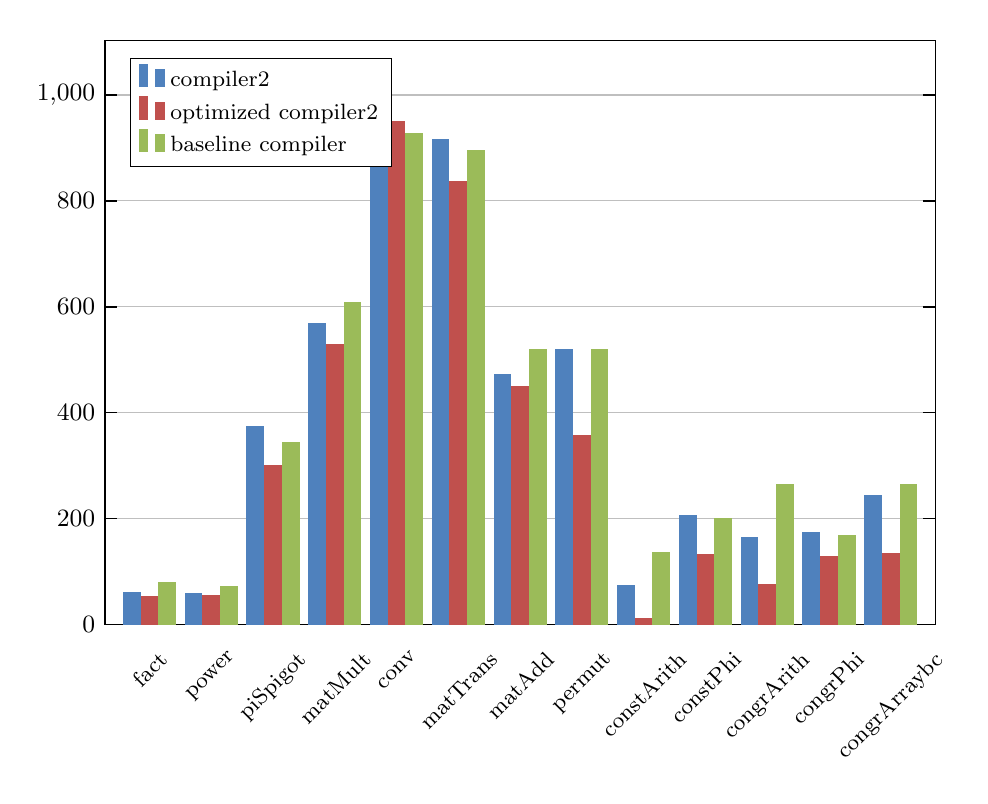
\begin{tikzpicture}
    \begin{axis}[
        width  = \textwidth,
        height = \chartheight,
        major x tick style = transparent,
        ybar=\barpadding,
        bar width=\barwidth,
        enlarge x limits=\enlargexlimits,
        ymajorgrids = true,
        tick style={semithick,color=black}, 
        symbolic x coords={fact,power,piSpigot,matMult,conv,matTrans,matAdd,permut,constArith,constPhi,congrArith,congrPhi,congrArraybc},
        xtick = data,
        scaled y ticks = false,
        ymin=0,
        legend cell align=left,
        legend pos=north west,
        legend style={font=\footnotesize},
		    tick label style = {font=\small},
		    x tick label style={rotate=45,font=\footnotesize},
    ]
    
%compiler2																										
\addplot[style={bblue,fill=bblue,mark=none}]																										
coordinates {(fact,	60	) (piSpigot,	374	) (power,	58	) (matMult,	569	) (matAdd,	472	) (matTrans,	915	) (conv,	1003	) (permut,	520	) (constArith,	74	) (constPhi,	205	) (congrArith,	164	) (congrPhi,	173	) (congrArraybc,	244	)};
																										
%optimized compiler2																										
\addplot[style={rred,fill=rred,mark=none}]																										
coordinates {(fact,	52	) (piSpigot,	300	) (power,	55	) (matMult,	528	) (matAdd,	449	) (matTrans,	836	) (conv,	949	) (permut,	357	) (constArith,	12	) (constPhi,	132	) (congrArith,	76	) (congrPhi,	128	) (congrArraybc,	133	)};
																										
%baseline compiler																										
\addplot[style={ggreen,fill=ggreen,mark=none}]																										
coordinates {(fact,	80	) (piSpigot,	344	) (power,	72	) (matMult,	608	) (matAdd,	520	) (matTrans,	896	) (conv,	928	) (permut,	520	) (constArith,	136	) (constPhi,	200	) (congrArith,	264	) (congrPhi,	168	) (congrArraybc,	264	)};


        \legend{compiler2,optimized compiler2,baseline compiler}
    \end{axis}
\end{tikzpicture}
\caption{Code size (bytes)}
\label{fig:code-size}
\end{figure}

\begin{figure}[H]
\centering
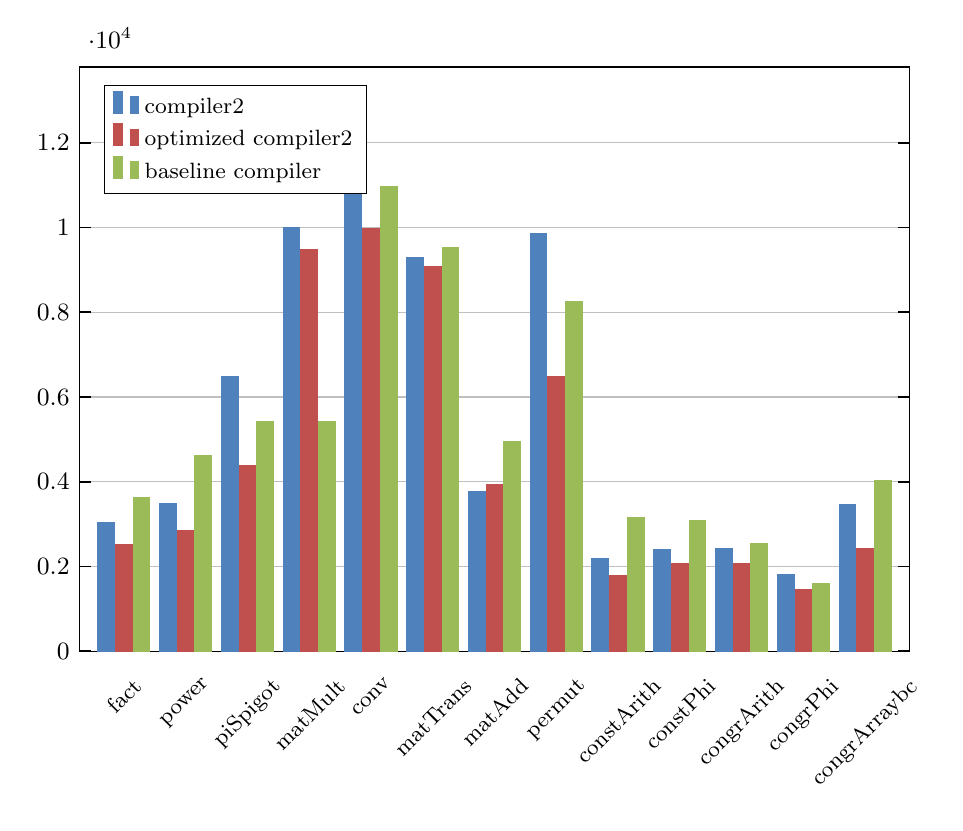
\begin{tikzpicture}
    \begin{axis}[
        width  = \textwidth,
        height = \chartheight,
        major x tick style = transparent,
        ybar=\barpadding,
        bar width=\barwidth,
        enlarge x limits=\enlargexlimits,
        ymajorgrids = true,
        tick style={semithick,color=black}, 
        symbolic x coords={fact,power,piSpigot,matMult,conv,matTrans,matAdd,permut,constArith,constPhi,congrArith,congrPhi,congrArraybc},
        xtick = data,
        scaled y ticks = false,
        ymin=0,
        legend cell align=left,
        legend pos=north west,
        legend style={font=\footnotesize},
		    tick label style = {font=\small},
		    x tick label style={rotate=45,font=\footnotesize},
	      y tick label style={/pgf/number format/fixed},
		    scaled y ticks=base 10:-4
    ]
    
%compiler2																										
\addplot[style={bblue,fill=bblue,mark=none}]																										
coordinates {(fact,	3045	) (piSpigot,	6490	) (power,	3487	) (matMult,	10003	) (matAdd,	3758	) (matTrans,	9288	) (conv,	12536	) (permut,	9851	) (constArith,	2189	) (constPhi,	2407	) (congrArith,	2413	) (congrPhi,	1814	) (congrArraybc,	3465	)};
																										
%optimized compiler2																										
\addplot[style={rred,fill=rred,mark=none}]																										
coordinates {(fact,	2512	) (piSpigot,	4376	) (power,	2841	) (matMult,	9481	) (matAdd,	3936	) (matTrans,	9080	) (conv,	9971	) (permut,	6491	) (constArith,	1779	) (constPhi,	2079	) (congrArith,	2061	) (congrPhi,	1451	) (congrArraybc,	2430	)};
																										
%baseline compiler																										
\addplot[style={ggreen,fill=ggreen,mark=none}]																										
coordinates {(fact,	3632	) (piSpigot,	5431	) (power,	4608	) (matMult,	5424	) (matAdd,	4950	) (matTrans,	9517	) (conv,	10979	) (permut,	8242	) (constArith,	3146	) (constPhi,	3074	) (congrArith,	2539	) (congrPhi,	1602	) (congrArraybc,	4034	)};


        \legend{compiler2,optimized compiler2,baseline compiler}
    \end{axis}
\end{tikzpicture}
\caption{Execution time ($\mu$sec)}
\label{fig:execution-time}
\end{figure}

\begin{figure}[H]
\centering
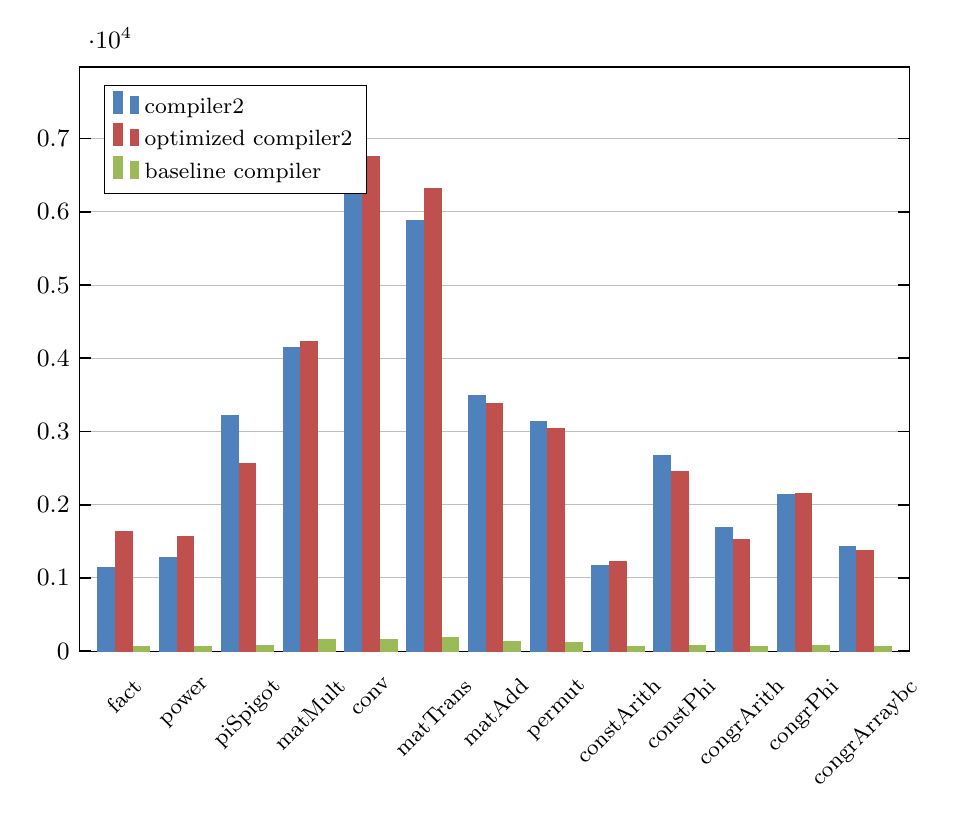
\begin{tikzpicture}
    \begin{axis}[
        width  = \textwidth,
        height = \chartheight,
        major x tick style = transparent,
        ybar=\barpadding,
        bar width=\barwidth,
        enlarge x limits=\enlargexlimits,
        ymajorgrids = true,
        tick style={semithick,color=black}, 
        symbolic x coords={fact,power,piSpigot,matMult,conv,matTrans,matAdd,permut,constArith,constPhi,congrArith,congrPhi,congrArraybc},
        xtick = data,
        scaled y ticks = false,
        ymin=0,
        legend cell align=left,
        legend pos=north west,
        legend style={font=\footnotesize},
		    tick label style = {font=\small},
		    x tick label style={rotate=45,font=\footnotesize},
		    scaled y ticks=base 10:-4
    ]
    
%compiler2																										
\addplot[style={bblue,fill=bblue,mark=none}]																										
coordinates {(fact,	1141	) (piSpigot,	3221	) (power,	1275	) (matMult,	4150	) (matAdd,	3493	) (matTrans,	5876	) (conv,	7253	) (permut,	3139	) (constArith,	1165	) (constPhi,	2668	) (congrArith,	1683	) (congrPhi,	2133	) (congrArraybc,	1425	)};
																										
%optimized compiler2																										
\addplot[style={rred,fill=rred,mark=none}]																										
coordinates {(fact,	1632	) (piSpigot,	2560	) (power,	1569	) (matMult,	4226	) (matAdd,	3377	) (matTrans,	6324	) (conv,	6755	) (permut,	3044	) (constArith,	1225	) (constPhi,	2451	) (congrArith,	1531	) (congrPhi,	2150	) (congrArraybc,	1371	)};
																										
%baseline compiler																										
\addplot[style={ggreen,fill=ggreen,mark=none}]																										
coordinates {(fact,	66	) (piSpigot,	82	) (power,	67	) (matMult,	164	) (matAdd,	135	) (matTrans,	182	) (conv,	154	) (permut,	117	) (constArith,	67	) (constPhi,	83	) (congrArith,	65	) (congrPhi,	81	) (congrArraybc,	64	)};


    \legend{compiler2,optimized compiler2,baseline compiler}
  \end{axis}
\end{tikzpicture}
\caption{Compilation time ($\mu$sec)}
\label{fig:compilation-time}
\end{figure}

\begin{table}[H]
\centering
\begin{tabular}{r r r r r r}
\toprule
~ & \multicolumn{3}{c}{Code size (\textit{bytes})} & \multicolumn{2}{c}{Ratio (\textit{\%})} \\
Benchmark & \textit{c2} & \textit{c2o} & \textit{bl} & \textit{c2o/c2} & \textit{c2o/bl} \\
\midrule
fact	 & 	60	 & 	52	 & 	80	 & 	86.7	 & 	65.0	 \\
piSpigot	 & 	374	 & 	300	 & 	344	 & 	80.2	 & 	87.2	 \\
power	 & 	58	 & 	55	 & 	72	 & 	94.5	 & 	76.1	 \\
matMult	 & 	569	 & 	528	 & 	608	 & 	92.8	 & 	86.9	 \\
matAdd	 & 	472	 & 	449	 & 	520	 & 	95.1	 & 	86.4	 \\
matTrans	 & 	915	 & 	836	 & 	896	 & 	91.4	 & 	93.3	 \\
conv	 & 	1003	 & 	949	 & 	928	 & 	94.7	 & 	102.3	 \\
permut	 & 	520	 & 	357	 & 	520	 & 	68.6	 & 	68.7	 \\
constArith	 & 	74	 & 	12	 & 	136	 & 	16.2	 & 	8.8	 \\
constPhi	 & 	205	 & 	132	 & 	200	 & 	64.3	 & 	65.9	 \\
congrArith	 & 	164	 & 	76	 & 	264	 & 	46.2	 & 	28.7	 \\
congrPhi	 & 	173	 & 	128	 & 	168	 & 	74.2	 & 	76.5	 \\
congrArraybc	 & 	244	 & 	133	 & 	264	 &	54.5	 & 	50.4	 \\
\bottomrule
\end{tabular}
\caption{Comparison of the size of compiled benchmark code produced by compiler2 (\textit{c2}), compiler2 with activated optimizations (\textit{c2o}) and baseline compiler (\textit{bl})}
\label{tab:evaluation:code-size}
\end{table}

\begin{table}[H]
\centering
\begin{tabular}{r R{1.1cm} R{1.1cm} R{1.1cm} r r}
\toprule
~ & \multicolumn{3}{c}{Execution time (\textit{$\mu$sec})} & \multicolumn{2}{c}{Ratio (\textit{\%})} \\
Benchmark & \textit{c2} & \textit{c2o} & \textit{bl} & \textit{c2o/c2} & \textit{c2o/bl} \\
\midrule
fact	 & 	3045	 & 	2512	 & 	3632	 & 	82.5	 & 	69.2	 \\
piSpigot	 & 	6490	 & 	4376	 & 	5431	 & 	67.4	 & 	80.6	 \\
power	 & 	3487	 & 	2841	 & 	4608	 & 	81.5	 & 	61.7	 \\
matMult	 & 	10003	 & 	9481	 & 	5424	 & 	94.8	 & 	174.8	 \\
matAdd	 & 	3758	 & 	3936	 & 	4950	 & 	104.7	 & 	79.5	 \\
matTrans	 & 	9288	 & 	9080	 & 	9517	 & 	97.8	 & 	95.4	 \\
conv	 & 	12536	 & 	9971	 & 	10979	 & 	79.5	 & 	90.8	 \\
permut	 & 	9851	 & 	6491	 & 	8242	 & 	65.9	 & 	78.8	 \\
constArith	 & 	2189	 & 	1779	 & 	3146	 & 	81.2	 & 	56.5	 \\
constPhi	 & 	2407	 & 	2079	 & 	3074	 & 	86.4	 & 	67.6	 \\
congrArith	 & 	2413	 & 	2061	 & 	2539	 & 	85.4	 & 	81.2	 \\
congrPhi	 & 	1814	 & 	1451	 & 	1602	 & 	80.0	 & 	90.6	 \\
congrArraybc	 & 	3465	 & 	2430	 & 	4034	 &	70.1	 & 	60.2	 \\
\bottomrule
\end{tabular}
\caption{Comparison of the execution time of compiled benchmark code produced by compiler2 (\textit{c2}), compiler2 with activated optimizations (\textit{c2o}) and baseline compiler (\textit{bl})}
\label{tab:evaluation:execution-time}
\end{table}

\begin{table}[H]
\centering
\begin{tabular}{r R{1.1cm} R{1.1cm} R{1.1cm} r r}
\toprule
~ & \multicolumn{3}{c}{Compilation time (\textit{$\mu$sec})} & \multicolumn{2}{c}{Ratio (\textit{\%})} \\
Benchmark & \textit{c2} & \textit{c2o} & \textit{bl} & \textit{c2o/c2} & \textit{c2o/bl} \\
\midrule
fact	 & 	1141	 & 	1632	 & 	66	 & 	143.1	 & 	2488.5	 \\
piSpigot	 & 	3221	 & 	2560	 & 	82	 & 	79.5	 & 	3129.6	 \\
power	 & 	1275	 & 	1569	 & 	67	 & 	123.0	 & 	2327.1	 \\
matMult	 & 	4150	 & 	4226	 & 	164	 & 	101.8	 & 	2582.6	 \\
matAdd	 & 	3493	 & 	3377	 & 	135	 & 	96.7	 & 	2496.3	 \\
matTrans	 & 	5876	 & 	6324	 & 	182	 & 	107.6	 & 	3467.0	 \\
conv	 & 	7253	 & 	6755	 & 	154	 & 	93.1	 & 	4398.7	 \\
permut	 & 	3139	 & 	3044	 & 	117	 & 	97.0	 & 	2593.8	 \\
constArith	 & 	1165	 & 	1225	 & 	67	 & 	105.1	 & 	1836.1	 \\
constPhi	 & 	2668	 & 	2451	 & 	83	 & 	91.9	 & 	2955.2	 \\
congrArith	 & 	1683	 & 	1531	 & 	65	 & 	91.0	 & 	2355.1	 \\
congrPhi	 & 	2133	 & 	2150	 & 	81	 & 	100.8	 & 	2648.3	 \\
congrArraybc	 & 	1425	 & 	1371	 & 	64	 & 	96.2	 & 	2132.3	 \\
\bottomrule
\end{tabular}
\caption{Comparison of the compilation time of compiler2 (\textit{c2}), compiler2 with activated optimizations (\textit{c2o}) and baseline compiler (\textit{bl})}
\label{tab:evaluation:compilation-time}
\end{table}

\begin{table}[H]
\centering
\begin{tabular}{r R{1.1cm} R{1.1cm} R{1.1cm} r r r}
\toprule
~ & \multicolumn{3}{c}{Compilation time (\textit{$\mu$sec})} & \multicolumn{3}{c}{Ratio (\textit{\%})} \\
Benchmark & \textit{de} & \textit{cfp} & \textit{gvn} & \textit{de/c2o} & \textit{cfp/c2o} & \textit{gvn/c2o} \\
\midrule
fact	 & 	18	 & 	11	 & 	44	 & 	1.1	 & 	0.7	 & 	2.7	 \\
piSpigot	 & 	55	 & 	25	 & 	147	 & 	2.2	 & 	1.0	 & 	5.7	 \\
power	 & 	16	 & 	10	 & 	45	 & 	1.0	 & 	0.6	 & 	2.9	 \\
matMult	 & 	55	 & 	30	 & 	167	 & 	1.3	 & 	0.7	 & 	3.9	 \\
matAdd	 & 	50	 & 	25	 & 	130	 & 	1.5	 & 	0.7	 & 	3.9	 \\
matTrans	 & 	114	 & 	53	 & 	289	 & 	1.8	 & 	0.8	 & 	4.6	 \\
conv	 & 	110	 & 	55	 & 	282	 & 	1.6	 & 	0.8	 & 	4.2	 \\
permut	 & 	60	 & 	25	 & 	144	 & 	2.0	 & 	0.8	 & 	4.7	 \\
constArith	 & 	40	 & 	24	 & 	107	 & 	3.3	 & 	2.0	 & 	8.7	 \\
constPhi	 & 	70	 & 	38	 & 	108	 & 	2.9	 & 	1.6	 & 	4.4	 \\
congrArith	 & 	40	 & 	18	 & 	114	 & 	2.6	 & 	1.1	 & 	7.4	 \\
congrPhi	 & 	52	 & 	23	 & 	104	 & 	2.4	 & 	1.1	 & 	4.8	 \\
congrArraybc	 & 	27	 & 	16	 & 	92	 & 	2.0	 & 	1.2	 & 	6.7	 \\
\bottomrule
\end{tabular}
\caption{Comparison of the time spent during dead code elimination (\textit{de}), constant folding/propagation (\textit{cfp}) and global value numbering (\textit{gvn}) (absolute numbers and ratio to total compilation time)}
\label{tab:evaluation:compilation-time-per-pass}
\end{table}

\begin{table}[H]
\centering
\begin{tabular}{r r r}
\toprule
~ & \multicolumn{2}{c}{Replaced nodes} \\
Benchmark & arithmetic & \irinline{PHIInst} \\
\midrule
fact	 & 	0	 & 	0	 \\
piSpigot	 & 	0	 & 	0	 \\
power	 & 	0	 & 	0	 \\
matMult	 & 	0	 & 	0	 \\
matAdd	 & 	0	 & 	0	 \\
matTrans	 & 	0	 & 	0	 \\
conv	 & 	0	 & 	0	 \\
permut	 & 	0	 & 	0	 \\
constArith	 & 	13	 & 	0	 \\
constPhi	 & 	4	 & 	5	 \\
congrArith	 & 	0	 & 	0	 \\
congrPhi	 & 	0	 & 	0	 \\
congrArraybc	 & 	0	 & 	0	 \\
\bottomrule
\end{tabular}
\caption{Nodes that could be replaced by \irinline{CONSTInst}s in the course of constant folding and constant propagation}
\label{tab:evaluation:constant-fold-prop}
\end{table}

\begin{table}[H]
\centering
\begin{tabular}{r r r r r}
\toprule
~ & \multicolumn{2}{c}{\irinline{CONSTInst}} & \multicolumn{2}{c}{arithmetic} \\
Benchmark & total & redundant & total & redundant \\
\midrule
fact	 & 	3	 & 	2	 & 	2	 & 	0	 \\
piSpigot	 & 	20	 & 	9	 & 	21	 & 	3	 \\
power	 & 	3	 & 	1	 & 	2	 & 	0	 \\
matMult	 & 	12	 & 	10	 & 	5	 & 	0	 \\
matAdd	 & 	9	 & 	7	 & 	3	 & 	0	 \\
matTrans	 & 	17	 & 	15	 & 	10	 & 	0	 \\
conv	 & 	19	 & 	17	 & 	11	 & 	0	 \\
permut	 & 	12	 & 	10	 & 	4	 & 	0	 \\
constArith	 & 	17	 & 	5	 & 	13	 & 	0	 \\
constPhi	 & 	25	 & 	17	 & 	5	 & 	2	 \\
congrArith	 & 	16	 & 	12	 & 	23	 & 	8	 \\
congrPhi	 & 	15	 & 	10	 & 	13	 & 	6	 \\
congrArraybc	 & 	8	 & 	6	 & 	0	 & 	0	 \\
\bottomrule
\end{tabular}
\\[6pt]
\begin{tabular}{r r r r r}
\toprule
~ & \multicolumn{2}{c}{\irinline{PHIInst}} & \multicolumn{2}{c}{array bounds-ch.} \\
Benchmark & total & redundant & total & redundant \\
\midrule
fact	 & 	2	 & 	0	 & 	0	 & 	0	 \\
piSpigot	 & 	4	 & 	0	 & 	0	 & 	0	 \\
power	 & 	2	 & 	0	 & 	0	 & 	0	 \\
matMult	 & 	4	 & 	0	 & 	9	 & 	0	 \\
matAdd	 & 	2	 & 	0	 & 	9	 & 	0	 \\
matTrans	 & 	7	 & 	0	 & 	16	 & 	3	 \\
conv	 & 	8	 & 	0	 & 	16	 & 	1	 \\
permut	 & 	4	 & 	0	 & 	12	 & 	6	 \\
constArith	 & 	0	 & 	0	 & 	0	 & 	0	 \\
constPhi	 & 	10	 & 	0	 & 	0	 & 	0	 \\
congrArith	 & 	0	 & 	0	 & 	0	 & 	0	 \\
congrPhi	 & 	6	 & 	2	 & 	0	 & 	0	 \\
congrArraybc	 & 	0	 & 	0	 & 	8	 & 	4	 \\
\bottomrule
\end{tabular}
\caption{Nodes detected as redundant by global value numbering}
\label{tab:evaluation:gvn}
\end{table}

\begin{table}[H]
\centering
\begin{tabular}{r r r}
\toprule
Benchmark & deleted & remaining \\
\midrule
fact	 & 	2	 & 	14	 \\
piSpigot	 & 	12	 & 	53	 \\
power	 & 	1	 & 	16	 \\
matMult	 & 	10	 & 	76	 \\
matAdd	 & 	7	 & 	68	 \\
matTrans	 & 	18	 & 	107	 \\
conv	 & 	18	 & 	117	 \\
permut	 & 	16	 & 	57	 \\
constArith	 & 	29	 & 	3	 \\
constPhi	 & 	26	 & 	47	 \\
congrArith	 & 	20	 & 	22	 \\
congrPhi	 & 	18	 & 	37	 \\
congrArraybc	 & 	10	 & 	18	 \\
\bottomrule
\end{tabular}
\caption{Dead nodes deleted during dead code elimination and remaining nodes in the program}
\label{tab:evaluation:dead-code-elimination}
\end{table}
\section{Related Work}
\label{sec:related}

Section \ref{sec:constantprop} introduced a simple algorithm which combines both constant folding and constant propagation. It discovers values which are statically known to be constant and uses this information to evaluate expressions at compile-time. Nevertheless, this optimization is based on assumptions which restrict the number of detected constant expressions. Basically, it supposes that all instructions in the program can be reached, but for an improvement of the optimization results, this assumption has to be dropped. What has to be considered is the evaluation of constant conditions. Obviously, if a result of a condition test can be computed at compile-time, it will be possible to gain information about which branches will never be executed during run-time. These unreachable code sections can then be ignored by further optimization and will be deleted from the program which is also referred to as \emph{unreachable code elimination} \cite{appel:2004:moderncompilerimpl}. Furthermore, the removal of conditional branches can have another positive effect, namely for the propagation of constants: The search for constants can now be restricted to the reachable branches which possibly yields propagation possibilities that have not been discovered before. Obviously, further propagation can raise additional potential regarding evaluation of condition tests which again could lead to the deletion of branches.

An approach  that combines both constant propagation and unreachable code elimination is followed by a technique called \emph{conditional constant propagation} \cite{wegman:1991:constantpropagation}. In contrast to the algorithm presented in section \ref{sec:constantprop}, it propagates values only to those code parts which are already known to be reachable. That means, based on symbolic execution, this optimization starts at the beginning of the program and continues by exploring which further code sections can be reached, where constant propagation will proceed. Wegman and Zadeck \cite{wegman:1991:constantpropagation} also give a formulation of this optimization which takes advantage of static single assignment form, called \emph{sparse conditional constant propagation}.

Another field, that offers various techniques yielding similar optimization results, regards the removal of redundancies in programs. This involves the discovery of equivalent expressions which, as mentioned earlier in section \ref{sec:global-value-numbering}, is known to be an undecidable problem. Besides the presented formulation of global value numbering, which discovers certain equivalencies based on the congruence of expressions, there exist a number of alternative techniques that strive to find preferably large portions of redundant computations. One of those techniques is referred to as \emph{partial redundancy elimination} which, in contrast to global value numbering, follows a lexical approach. This means, it identifies expressions that are textually congruent and allows for discovery of redundant computations which are not necessarily value-congruent \cite{click:1995:combininganalyses}.
The scope of this optimization spans the detection and removal of redundancies which occur along some but not necessarily along all paths through a program. These are also referred to as \emph{partial redundancies} \cite{aho:2006:compilersprinciples}.
More generally, it also detects \emph{common sub-expressions} and \emph{loop-invariant code} which can be viewed as special types of partial redundancies. Once this optimization has discovered redundant computations, it will delete or relocate the according expressions, so that they will be evaluated only as often as necessary during execution of the program.

In general, the portions of redundancies found by global value numbering and partial redundancy elimination are overlapping, however, the two optimizations do not find exactly the same equivalencies. According to Click \cite{click:1995:gcm-gvn}, in practice, global value numbering can be expected to find more redundancies than partial redundancy elimination. Approaches exist that try to combine both techniques to maximize the number of detected redundant expressions \cite{vandrunen:2004:pre-gvn}.
\section{Conclusions}
\label{sec:conclusions}

In this thesis we presented machine-independent optimizations for use within the new optimizing compiler of the CACAO VM. Dead code elimination, constant folding, constant propagation and global value numbering have been described and it has been shown how they can be applied to the SSA-based intermediate representation of the compiler. Due to the characteristics of this intermediate representation, constant propagation becomes an implicit effect of constant folding, hence both techniques can be combined in a single compiler pass. The program transformations in the course of constant folding, constant propagation as well as global value numbering inherently lead to dead code and thus have to be followed by a run of dead code elimination.

Based on our examinations the optimizations have been implemented and added to the compiler. Thereby, the code size as well as the execution time of compiled programs could be decreased which mainly can be attributed to global value numbering. Though compilation time has slightly increased on average, in some cases the optimizations also achieve faster compilation, since less work has to be done within subsequent compiler passes.


\newpage

\appendix
\section{Alpern et al.'s Partitioning Algorithm}
\label{sec:alpern-partitioning}

In section \ref{sec:global-value-numbering:application-to-the-ir} we presented an algorithm for the partition refinement process of global value numbering. Alpern et al.\ \cite{alpern:1988:detecting-equality-of-variables} presented an according algorithm, which is also inspired by Hopcroft's algorithm for minimizing the number of states of a finite automaton. In fact, they do not use the original version of this algorithm, instead they base their work on a reformulation given by Aho et al.\ \cite{aho:1974:the-design-and-analysis-of-computer-algorithms}.

In their explanations Alpern et al.\ use an intermediate representation referred to as \emph{value graph}, which is very similar to that one used by CACAO's new compiler framework. Basically, expressions or operations are represented by nodes, the dependencies of the corresponding values are modeled by edges. Each node is labeled with a function symbol, describing the kind of operation it represents. Two nodes in this graph are said to be \emph{congruent} if the following prerequisites hold:
\begin{itemize}
\item The nodes have identical function labels.
\item The corresponding destinations of the edges leaving the nodes are congruent.
\end{itemize}
Furthermore, the term congruence is defined as the maximal fixed point which satisfies these conditions.

\begin{algorithm}[H]
\caption{Alpern et al.'s partitioning algorithm}
\label{alg:alpern-partitioning}
\begin{algorithmic}[1]
\State $\mathit{WAITING} \leftarrow \lbrace 1, 2, \ldots , p\rbrace$
\State $q \leftarrow p$
\While{$\mathit{WAITING} \neq \emptyset$}
	\State select and delete an integer $i$ from $\mathit{WAITING}$
	\For{$m$ from $1$ to $k$}\label{alg:alpern-partitioning:operand-index-loop}
		\State $\mathit{INVERSE} \leftarrow \emptyset$
		\For{$x$ in $B[i]$}
			\State $\mathit{INVERSE} \leftarrow \mathit{INVERSE}\cup F^{-1}[m, x]$
		\EndFor
		\For{each $j$ such that $B[j]\cap \mathit{INVERSE} \neq \emptyset$ and $B[j] \not\subseteq \mathit{INVERSE}$}\label{alg:alpern-partitioning:inverse-loop}
			\State $q \leftarrow q + 1$
			\State create a new block $B[q]$
			\State $B[q] \leftarrow B[j] \cap \mathit{INVERSE}$
			\State $B[j] \leftarrow B[j] - B[q]$
			\If{$j$ is in $\mathit{WAITING}$}\label{alg:alpern-partitioning:if-in-waiting}
				\State add $q$ to $\mathit{WAITING}$
			\Else
				\If{$|B[j]| \leq |B[q]|$}
					\State add $j$ to $\mathit{WAITING}$
				\Else
					\State add $q$ to $\mathit{WAITING}$
				\EndIf
			\EndIf
		\EndFor
	\EndFor
\EndWhile
\end{algorithmic}
\end{algorithm}

Based on these considerations it is now possible to create an initial partitioning of the nodes into blocks. According to the process described in section \ref{sec:global-value-numbering:application-to-the-ir}, at the beginning of this optimization all nodes with identical function labels are assumed to be congruent and therefore, they are put in the same block. For the subsequent refinement of these blocks, the corresponding process, as formulated by Alpern et al., is presented in algorithm \ref{alg:alpern-partitioning}. It takes as input the initial partitioning of nodes into blocks and a set of functions $f_i$ where $f_i(x)$ denotes the node that serves as $i$th operand for $x$. The partitioning of the nodes is represented by a vector denoted by $B$, which contains blocks of nodes. Instead of blocks, the work list $\mathit{WAITING}$ holds indices, which are used to refer to the corresponding elements in $B$. Furthermore the algorithm uses a mapping $F^{-1}$ so that $F^{-1}[m,x]$ denotes the set of nodes that use $x$ as their $m$th operand, namely, $F^{-1}[m,x]$ represents the inverse image of node $x$ under $f_m$.

Problems arise with this algorithm when an integer $i$ is picked from the work list, so that at some iteration of the loop starting at line \ref{alg:alpern-partitioning:operand-index-loop}, it holds that the condition $B[j]\cap \mathit{INVERSE} \neq \emptyset$ and $B[j] \not\subseteq \mathit{INVERSE}$ at line \ref{alg:alpern-partitioning:inverse-loop} is true for $j = i$. According situations can cause that at termination of the algorithm, non-congruent nodes are in the same block.

\begin{figure}[H]
\centering
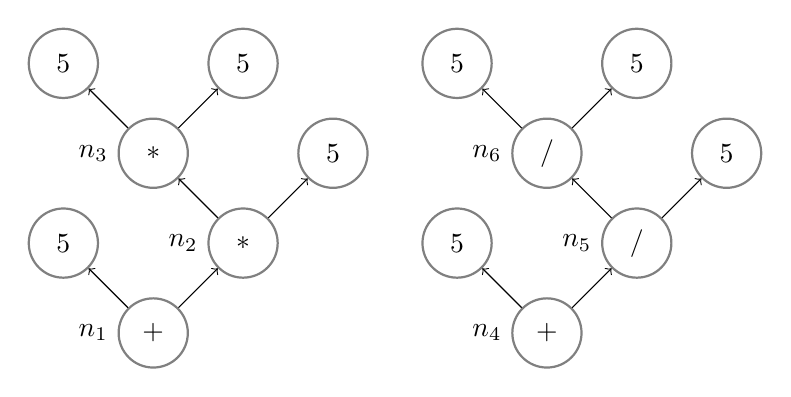
\begin{tikzpicture}
[
hidden/.style={
	draw=black,
	node distance=5cm and 5cm,
	minimum width=100pt
},
value/.style={
	circle,
	draw=black!50,
	thick,
	minimum size=25pt,
	inner sep=0pt,
	node distance=0.5cm and 0.5cm,
	align=center}
]
  
  \node[value, label=left:$n_1$] (add1) at (-5,0) {$+$};
  \node[value] (const1) [above left=of add1] {$5$};
  \node[value, label=left:$n_2$] (mul1) [above right=of add1] {$*$};
  \node[value, label=left:$n_3$] (mul2) [above left=of mul1] {$*$};
  \node[value] (const2) [above right=of mul1] {$5$};
  \node[value] (const3) [above left=of mul2] {$5$};
  \node[value] (const4) [above right=of mul2] {$5$};
  
  \node[value, label=left:$n_4$] (add2) {$+$};
  \node[value] (const5) [above left=of add2] {$5$};
  \node[value, label=left:$n_5$] (div1) [above right=of add2] {$/$};
  \node[value, label=left:$n_6$] (div2) [above left=of div1] {$/$};
  \node[value] (const6) [above right=of div1] {$5$};
  \node[value] (const7) [above left=of div2] {$5$};
  \node[value] (const8) [above right=of div2] {$5$};
  % edges
  \draw [->] (add1) to (const1);
  \draw [->] (add1) to (mul1);
  \draw [->] (mul1) to (mul2);
  \draw [->] (mul1) to (const2);
  \draw [->] (mul2) to (const3);
  \draw [->] (mul2) to (const4);
  
  \draw [->] (add2) to (const5);
  \draw [->] (add2) to (div1);
  \draw [->] (div1) to (div2);
  \draw [->] (div1) to (const6);
  \draw [->] (div2) to (const7);
  \draw [->] (div2) to (const8);
\end{tikzpicture}
\caption{}
\label{fig:alpern-partitioning-counterexample}
\end{figure}

Figure \ref{fig:alpern-partitioning-counterexample} shows a value graph which in turn comprises two sub-graphs representing two independent expressions (this example is illustrated based on the notation used by Alpern et al.\ \cite{alpern:1988:detecting-equality-of-variables}, where data dependencies are modeled by arrows pointing in use-def direction). Obviously nodes $n_1$ and $n_4$ are not congruent because the operands $n_2$ and $n_5$ have distinct function labels. Accordingly, both nodes should be placed in different blocks at the end of the algorithm. We will show in the following, that there exists a possible execution sequence, so that $n_1$ and $n_4$ will reside in the same block. Assume that after the initial partitioning, the blocks are defined as follows:

\vspace{-10pt}
\begin{align*}
B[1] &= \lbrace n_2,n_3\rbrace\\
B[2] &= \lbrace n_5,n_6\rbrace\\
B[3] &= \lbrace n_1,n_4\rbrace\\
B[4] &= \text{nodes with constant value } 5
\end{align*}

At the beginning of the algorithm, $\textit{WAITING}$ is initialized to $\lbrace 1, 2, 3, 4\rbrace$. Without loss of generality, assume that at the first iteration of the while loop, the integer $1$ is picked from $\textit{WAITING}$. The algorithm continues at the loop in line \ref{alg:alpern-partitioning:operand-index-loop} for $m = 1$ and computes the union of the inverse images for all nodes in $B[1]$ under $f_1$, leading to $\textit{INVERSE} = \lbrace n_2\rbrace$. Obviously, at line \ref{alg:alpern-partitioning:inverse-loop}, the condition in the loop header is true only for $j = 1$. Accordingly, a new block $B[5] = \lbrace n_2\rbrace$ will be created and the node $n_2$ is removed from $B[1]$. Since $1$ is not in the $\textit{WAITING}$ set anymore and $|B[1]| \leq |B[5]|$, $1$ will be added to $\textit{WAITING}$ again (see lines \ref{alg:alpern-partitioning:if-in-waiting} et seqq.). At the next iteration of the outmost for-loop (for $m = 2$), the set $B[1]$ will only contain the node $n_3$, thus, there will not happen any changes to the blocks.

For the next iteration of the while loop, we assume, without loss of generality, that the integer $2$ is selected from the work list. The following execution of the loop body will proceed similar to the previous iteration described above. Accordingly, there will be created a new block $B[6] = \lbrace n_5\rbrace$ and $B[2]$ will be changed to only contain $n_6$. Furthermore, $2$ will be added to $\textit{WAITING}$, which will then contain $1$, $2$, $3$ and $4$.

In subsequent iterations, the algorithm will select and delete all the remaining indices in $\textit{WAITING}$ but no further changes to the blocks will be applied. Thus, at termination, $B$ will contain the following blocks:

\vspace{-10pt}
\begin{align*}
B[1] &= \lbrace n_3\rbrace \\
B[2] &= \lbrace n_6\rbrace \\
B[3] &= \lbrace n_1,n_4\rbrace \\
B[4] &= \text{nodes with constant value } 5 \\
B[5] &= \lbrace n_2\rbrace \\
B[6] &= \lbrace n_5\rbrace
\end{align*}

As claimed above, the nodes $n_1$ and $n_4$ are contained in one common block. Thus, the algorithm yields an incorrect partitioning.

\newpage

\bibliography{references}

\end{document}
